% Created 2019-09-22 Sun 14:21
% Intended LaTeX compiler: pdflatex
\documentclass[10pt,t]{beamer}
\usepackage[utf8]{inputenc}
\usepackage[T1]{fontenc}
\usepackage{graphicx}
\usepackage{grffile}
\usepackage{longtable}
\usepackage{wrapfig}
\usepackage{rotating}
\usepackage{amsmath}
\usepackage{textcomp}
\usepackage{amssymb}
\usepackage{capt-of}
\usepackage{hyperref}
\usetheme{default}
\author{L. Larrabee Strow}
\date{\today}
\title{\large AIRS Calibration for Climate Trend Studies: Status and Future}
\subtitle{\footnotesize{AIRS Science Team Meeting}}
\date{\vspace{0.1in}\footnotesize{\today\vfill}}
\author{L. Larrabee Strow\inst{1,2}}
\institute[UMBC]{\inst{1} UMBC Physics Dept. \and \inst{2}UMBC JCET}
\input beamer_setup
\usetheme{metropolis}
\metroset{titleformat title=allcaps}
\renewcommand{\UrlFont}{\small\tt}
\renewcommand*{\UrlFont}{\footnotesize}
\tolerance=1000
\RequirePackage{fancyvrb}
\DefineVerbatimEnvironment{verbatim}{Verbatim}{fontsize=\footnotesize}
\begin{document}

\maketitle
\addtobeamertemplate{block begin}{
  \setlength{\parsep}{0pt}
  \setlength{\topsep}{3pt plus 2pt minus 2.5pt}
  \setlength{\itemsep}{0pt plus 0pt minus 2pt}
  \setlength{\partopsep}{2pt}
}


\begin{frame}[label={sec:orgec4751a},shrink=30]{Calibration Requirements for Climate Science}
\vspace{-0.1in}
\begin{large}
\begin{itemize}
\item AIRS 17+ year record long enough to address key climate questions
\item Stability of radiometric calibration is key
\item AIRS sensitivity to \cd, SST, etc allows stringent tests of stability
\end{itemize}
\end{large}
\vspace{-0.2in}
\begin{columns}
\begin{column}{0.55\columnwidth}
\begin{block}{Climate Science Questions}
\vspace{0.05in}
\emph{All require min \textasciitilde{}0.1K/decade stability}
\vspace{-0.05in}
\begin{itemize}
\item Global Trending: T(z), \water(z), T\textsubscript{surf}
\item Water vapor feedback (Does relative humidity vary)
\item Cloud feedback
\item Trends in PBL cloud occurance
\item OLR anomalies separated by cause: T/\water/cloud/surface, etc.
\end{itemize}
\end{block}
\end{column}

\begin{column}{0.55\columnwidth}
\begin{block}{Hyperspectral IR Advantages}
\begin{itemize}
\item AIRS senses both climate forcings, and responses
\item Clean separation of tropospheric vs stratospheric temperature trends (unlike microwave)
\item Multiple long-term overlapping missions (AIRS, CrIS, IASI)
\item AIRS, CrIS, IASI aleady agree to \textasciitilde{}0.1-0.3K and can be merged to 0.03K or better.
\end{itemize}
\end{block}
\end{column}
\end{columns}



\vspace{0.2in}
\begin{large}
Significant AIRS calibration drifts have \alert{already} resulted publication of in-accurate data that were publized by NASA/GSFC and the media (Washington Post, Scientific American).  \emph{This talk suggests how to make AIRS an accurate instrument for climate science.}
\end{large}
\end{frame}

\begin{frame}[label={sec:org36c1f28},shrink=20]{Weather versus Climate Research}
\begin{block}{Weather Applications}
\begin{itemize}
\item AIRS original focus was for NWP
\item Both 1Dvar retrievals and data assimilation \emph{require} bias removal
\begin{itemize}
\item NWP: biases due to the instrument, RTA, model
\item Retrievals: biases due to the instrument and RTA
\item Bias removal is generally in the \textasciitilde{}0.1-0.3K range
\end{itemize}
\item Radiometric accuracy is important
\begin{itemize}
\item But, below the nominal \textasciitilde{}0.3K range we cannot differentiate instrument vs RTA errors.
\item Spectroscopy errors are at the 1-2\% level, or 0.1-0.3K
\end{itemize}
\end{itemize}
\end{block}
\begin{block}{Climate Applications}
\begin{itemize}
\item Anomalies are the main language of climate observations
\item Although energy budget and fluxes are important, AIRS is not a major contributor
\item For AIRS, radiometric stability is most fundamental calibration requirement
\end{itemize}

Hyperspectral IR instrument stability appears to be 1-2 orders of magnitude better than absolute accuracy.  This is where we can shine, especially with a 17+ year record.
\end{block}
\end{frame}

\begin{frame}[label={sec:orga253539},shrink=5]{Climate Product Characteristics}
\begin{block}{Uncertainty Estimates}
\begin{itemize}
\item If we provide something unique, validation will be difficult
\item Internal product uncertainty estimates will be far more important than for weather applciations
\item Establishing uncertainites for products is a NASA ROSES requirement!
\end{itemize}
\end{block}

\begin{block}{Reproducibility}
\begin{itemize}
\item Reproducibiity of results is becoming increasingly important
\item Difficlt to achieve with our Level 2 approach
\item For climate simpler algorithms with reproducible results would enhance our impact on the broader community
\end{itemize}

There is a long history of controversies in climate measurements (esp. microwave temperature trends).  AIRS derived results will be heavily scrutinized, we need to be prepared for that to retain trust.
\end{block}
\end{frame}

\begin{frame}[label={sec:org081e89d}]{AIRS Stability Calibration: An Approach}
\begin{itemize}
\item External standards needed to establish stability
\item \cd and possibly \nitrous and \methane can provide those standards
\begin{itemize}
\item \cd is well mixed (on long time scales) and extremely well known
\item Establish AIRS stability by retrieving \cd anomalies (vs time)
\end{itemize}
\item SST is the other well established climate record
\begin{itemize}
\item Similarly, use retrieved SST anomalies to test AIRS stability
\end{itemize}
\item Land surface temperatures are another possibility, although less reliable than SST but of great interest and heavily studied.
\end{itemize}

Essentially you need to perform climate-level retrievals to test the capabilities of your instrument.  

A \emph{key} requirement is the need to reprocess the \emph{full record} many times.  NOT possible with Level 2 approach!  Need fast alternatives that may also address issues of reproducibility.
\end{frame}

\begin{frame}[label={sec:org8b01e67}]{Characteristics of AIRs Long-Term Radiance Trends}
\begin{itemize}
\item 1\% random subset
\end{itemize}
\end{frame}
\begin{frame}[label={sec:orgfef225e}]{AIRS Global 16-Year B(T) Trend}
All channels (including fill)

\begin{center}
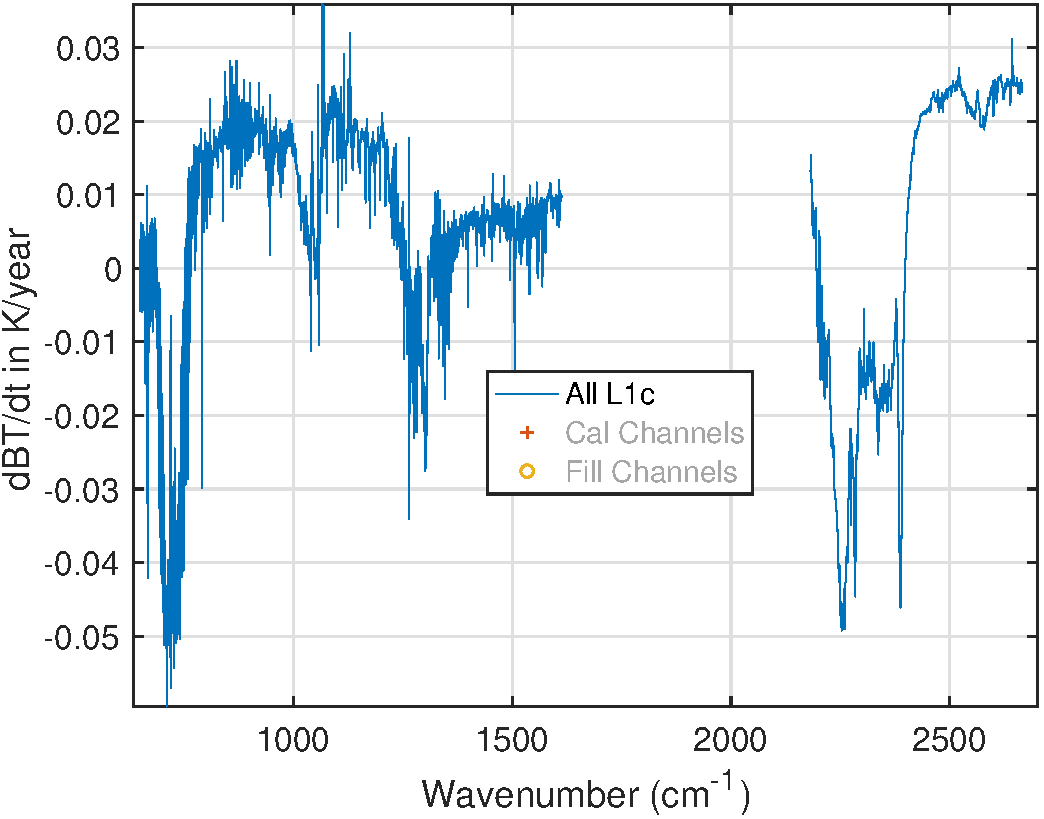
\includegraphics[width=0.85\linewidth]{./Figs/Pdf/rand_global_trend_l1c_overview.pdf}
\end{center}
\end{frame}

\begin{frame}[label={sec:org7c679e3}]{AIRS Global 16-Year B(T) Trend}
Fill channels marked

\begin{center}
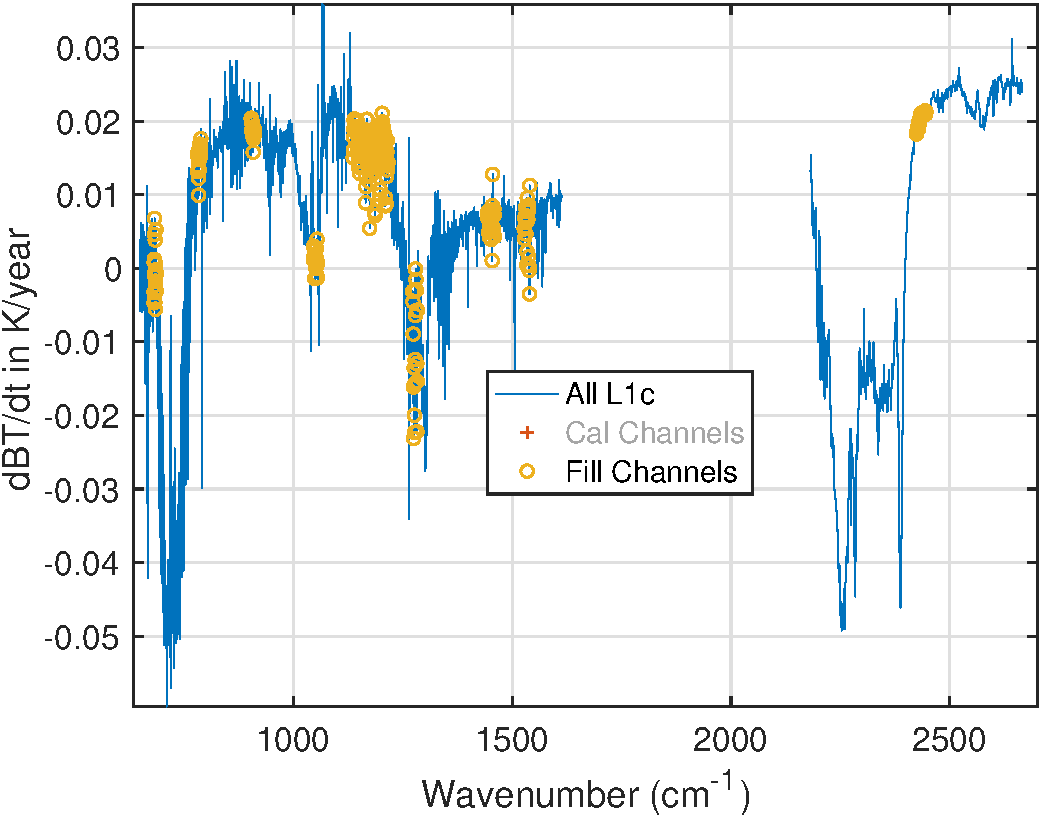
\includegraphics[width=0.85\linewidth]{./Figs/Pdf/rand_global_trend_l1c_overview_fill_marked.pdf}
\end{center}
\end{frame}

\begin{frame}[label={sec:org58f8280}]{AIRS Global 16-Year B(T) Trend}
\vspace{-0.1in}

\begin{center}
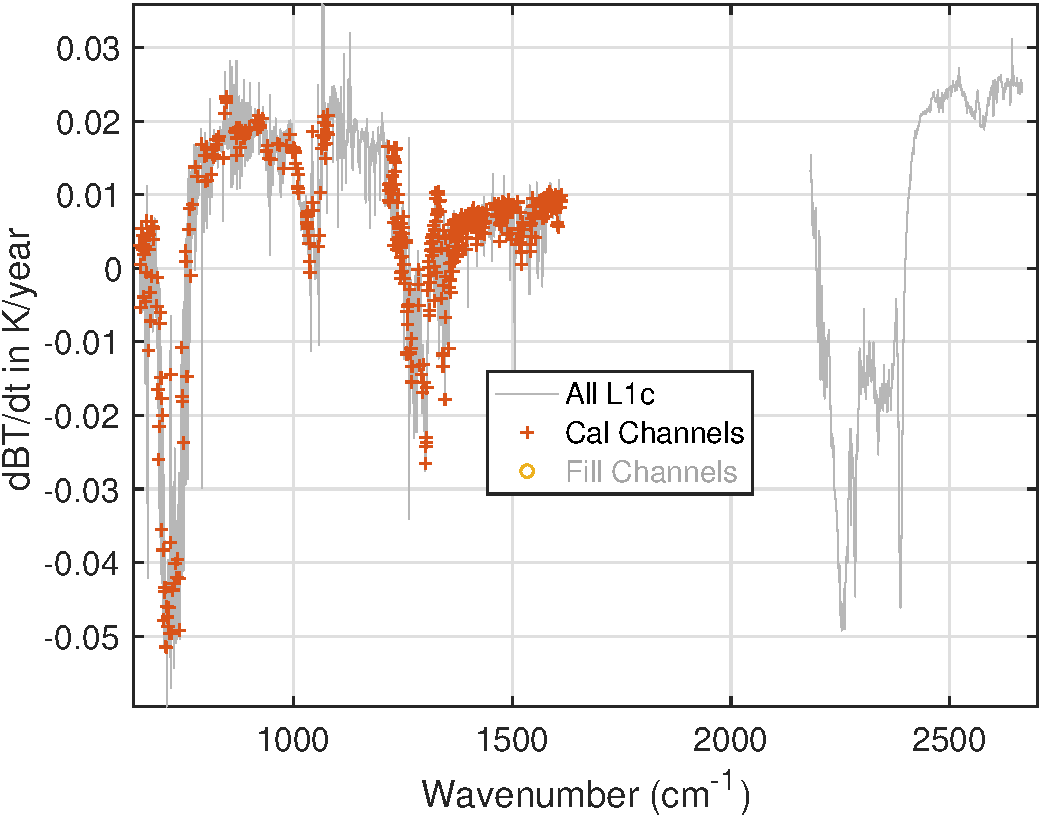
\includegraphics[width=0.75\linewidth]{./Figs/Pdf/rand_global_trend_l1c_overview_calfit_marked.pdf}
\end{center}

\vspace{-0.15in}
\begin{footnotesize}
\begin{itemize}
\item Channels used for calibration testing marked.
\item These channels have no A/B state changes, good S/N, small drift
\item Note sparsity of \cd channels in tropospheric sounding region
\end{itemize}
\end{footnotesize}
\end{frame}

\begin{frame}[label={sec:org4df7eb4}]{\cd and \methane Trends Removed, Fitted Chans Only}
\begin{center}
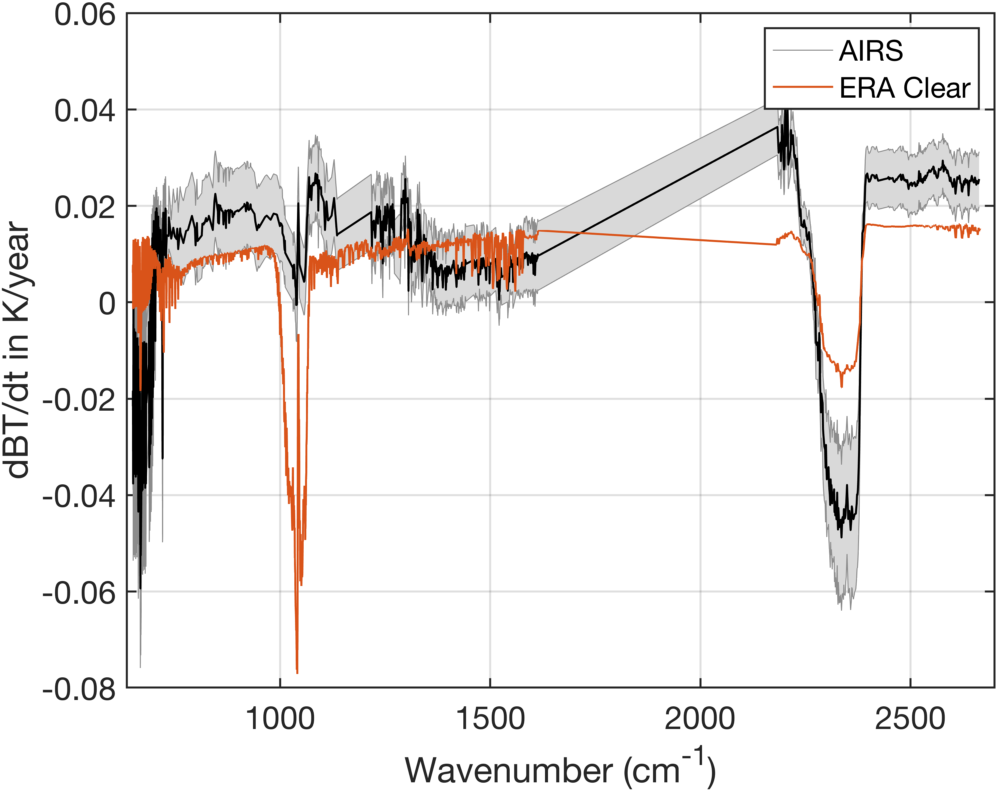
\includegraphics[width=0.75\linewidth]{./Figs/Png/rand_global_trend_l1c_vs_era_clr_only_fit_chans.png}
\end{center}

Uncertainty (gray) is geophysical (Std over latitutde).
\end{frame}

\begin{frame}[label={sec:orgc68a3b9}]{BT Response to Constant Relative Humidity}
\begin{center}
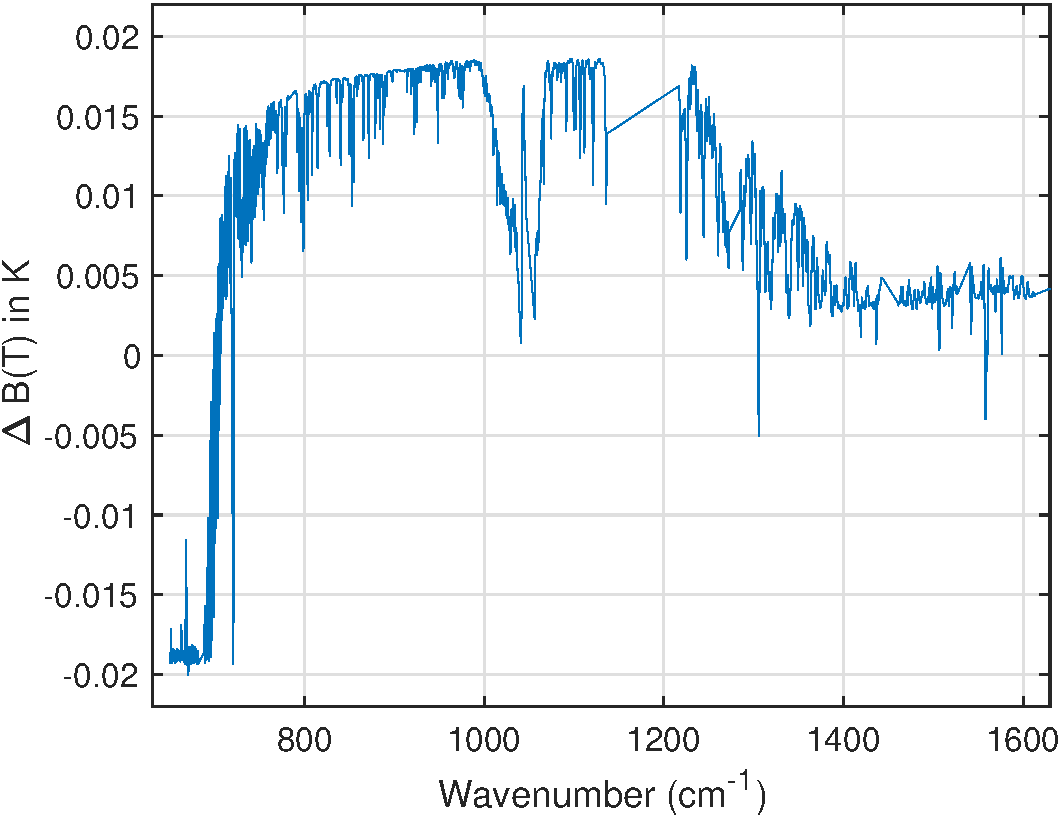
\includegraphics[width=0.7\linewidth]{./Figs/Pdf/dbt_constantRH_dsurf_dtrop=0.02k_dstrat=m0.02k.pdf}
\end{center}
\end{frame}
\begin{frame}[label={sec:org0b88e23}]{Retrieval of \cd, \nitrous, \methane Anomalies}
\begin{itemize}
\item oem approach
\item data set
\end{itemize}
\end{frame}
\begin{frame}[label={sec:org4cd4520}]{Pdf/raw\_co2\_vs\_era\_co2\_example\_lati28\_mlo\_lat.pdf}
\begin{center}
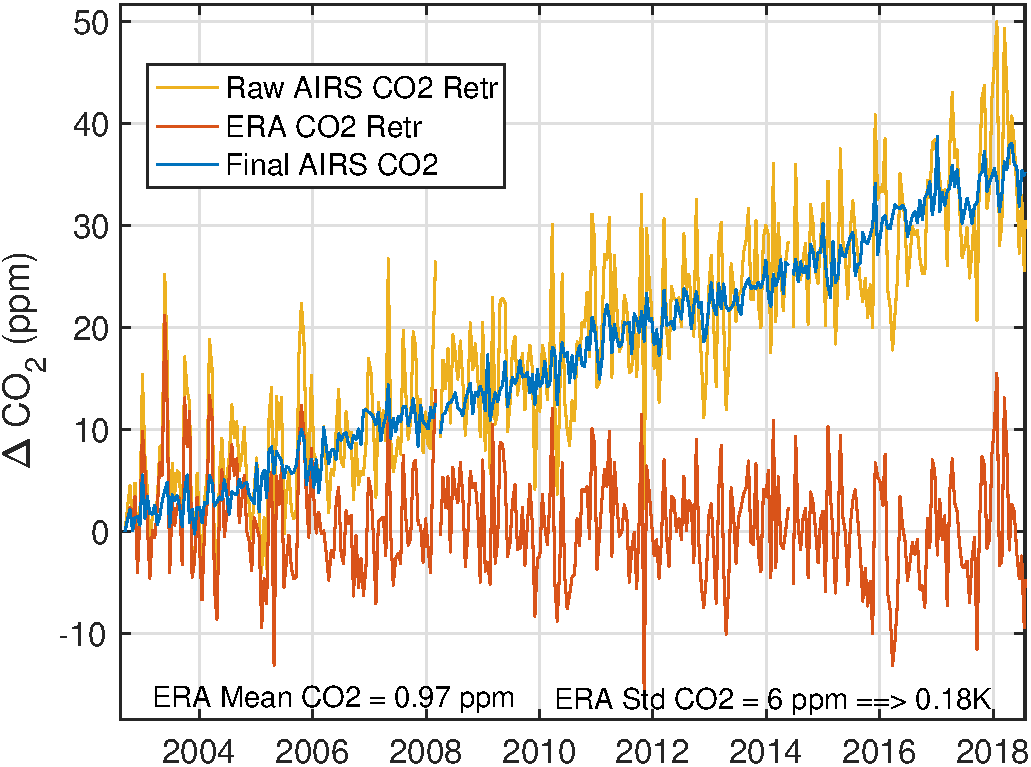
\includegraphics[width=0.7\linewidth]{./Figs/Pdf/raw_co2_vs_era_co2_example_lati28_mlo_lat.pdf}
\end{center}
\end{frame}

\begin{frame}[label={sec:org71fd442}]{Pdf/co2\_airs\_vs\_esrl\_global\_with\_dbt.pdf}
\begin{center}
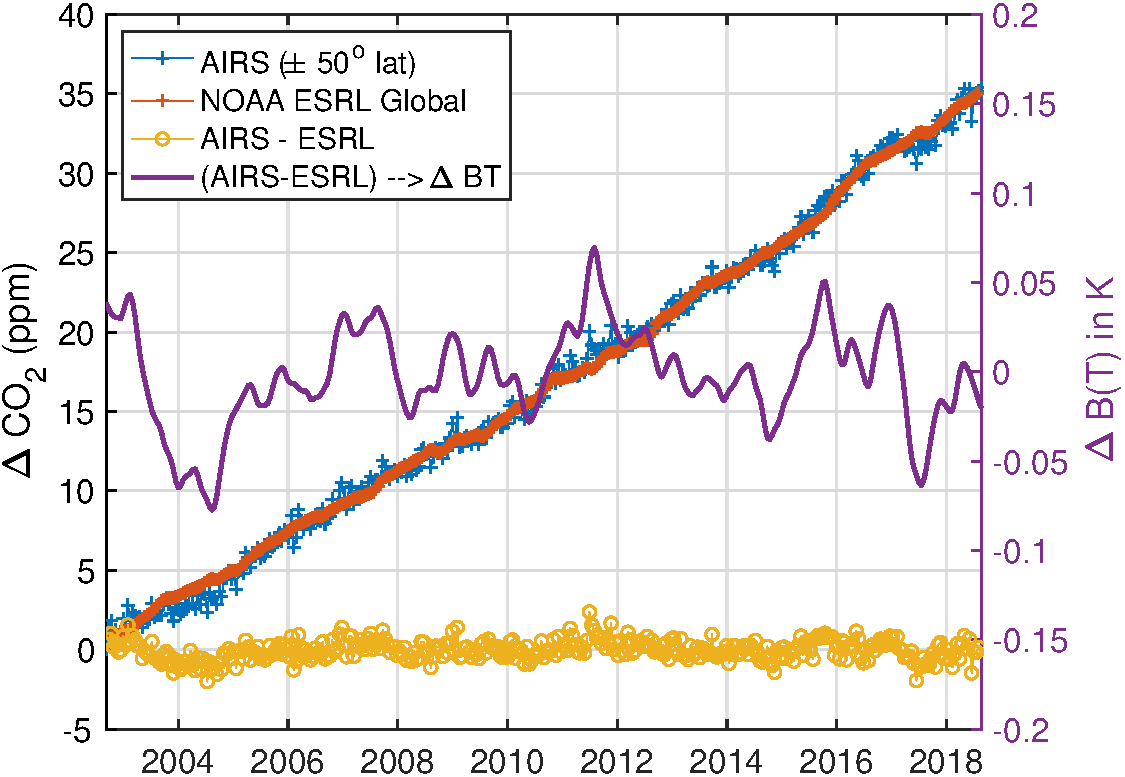
\includegraphics[width=0.7\linewidth]{./Figs/Pdf/co2_airs_vs_esrl_global_with_dbt.pdf}
\end{center}
\end{frame}

\begin{frame}[label={sec:org8623bf5}]{Pdf/co2\_airs\_vs\_mlo.pdf}
\begin{center}
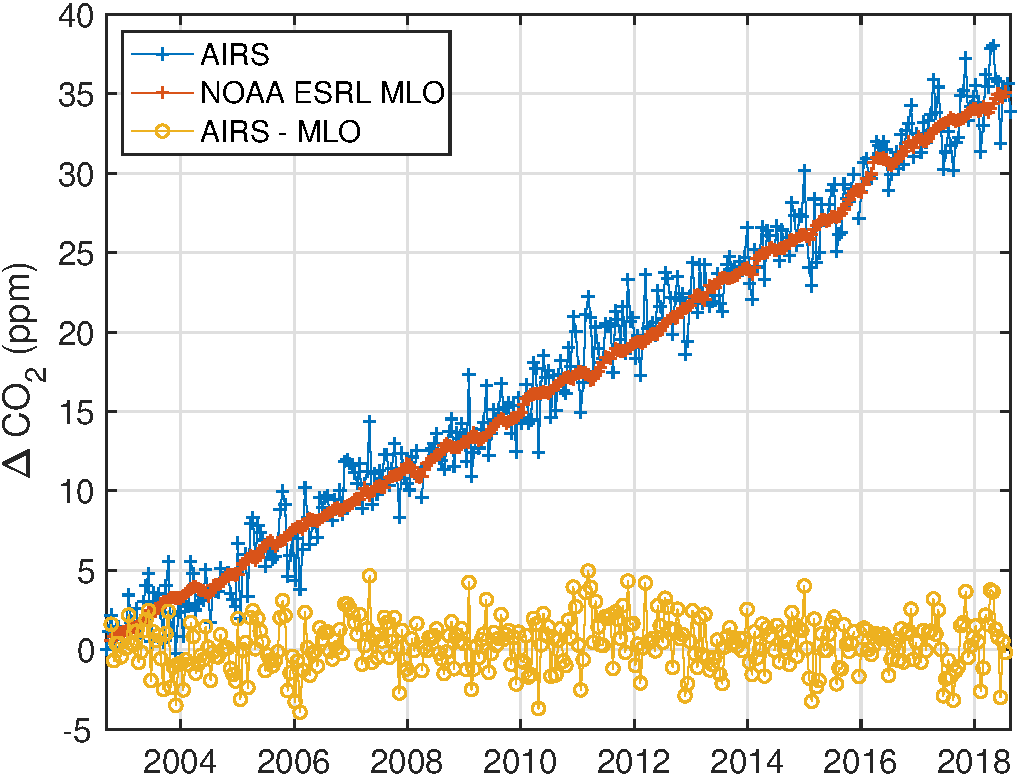
\includegraphics[width=0.7\linewidth]{./Figs/Pdf/co2_airs_vs_mlo.pdf}
\end{center}
\end{frame}

\begin{frame}[label={sec:org0b480aa}]{Pdf/co2\_growth\_vs\_lat.pdf}
\begin{center}
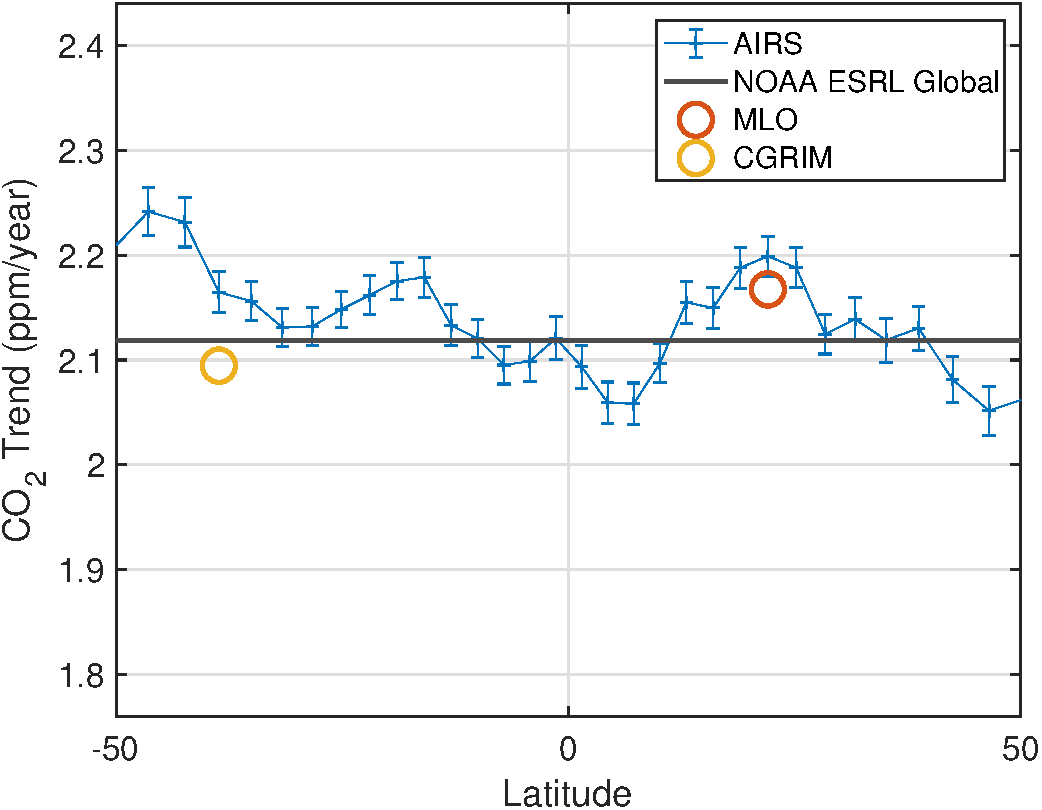
\includegraphics[width=0.7\linewidth]{./Figs/Pdf/co2_growth_vs_lat.pdf}
\end{center}
\end{frame}

\begin{frame}[label={sec:orge350b67}]{Pdf/co2\_airs\_vs\_esrl\_global\_growth\_anom.pdf}
\begin{center}
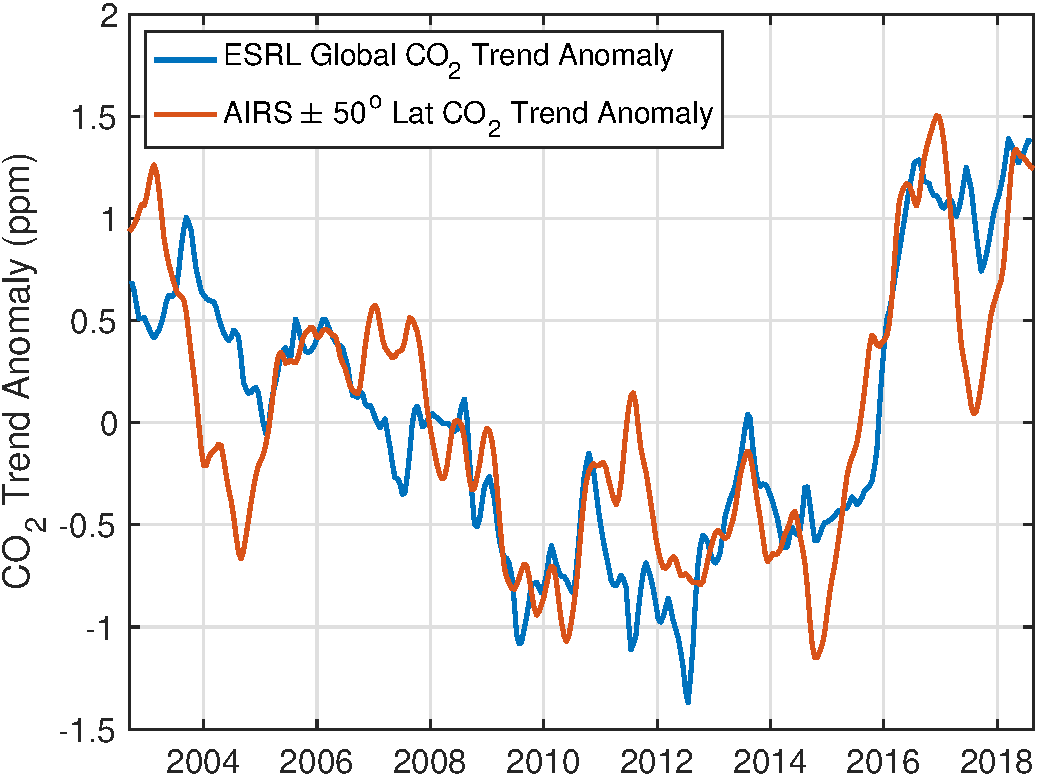
\includegraphics[width=0.7\linewidth]{./Figs/Pdf/co2_airs_vs_esrl_global_growth_anom.pdf}
\end{center}
\end{frame}

\begin{frame}[label={sec:org3ab2171}]{Png/co2\_anom\_image\_lat\_vs\_time.png}
\begin{center}
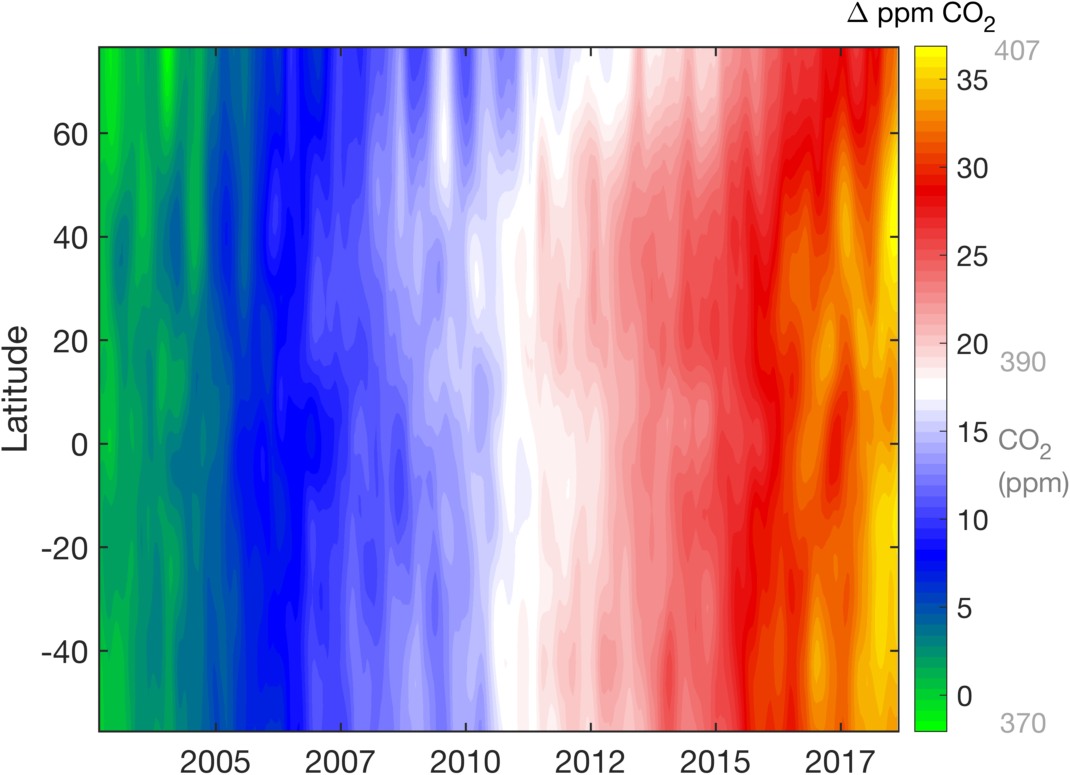
\includegraphics[width=0.7\linewidth]{./Figs/Png/co2_anom_image_lat_vs_time.png}
\end{center}
\end{frame}

\begin{frame}[label={sec:orgc53cace}]{Png/co2\_anomaly\_image\_fancy2\_corrected.png}
\begin{center}
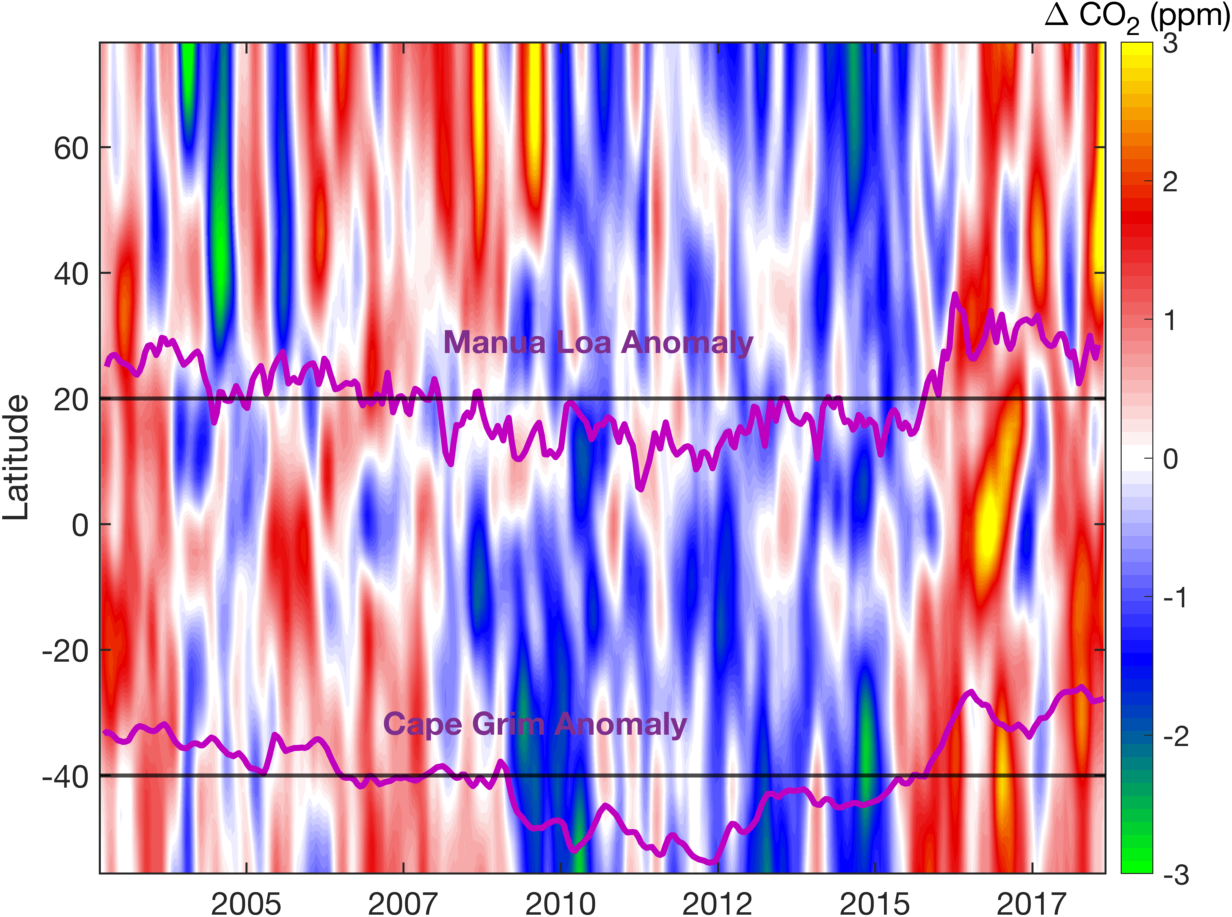
\includegraphics[width=0.7\linewidth]{./Figs/Png/co2_anomaly_image_fancy2_corrected.png}
\end{center}
\end{frame}

\begin{frame}[label={sec:org41451de}]{Pdf/n2o\_airs\_vs\_esrl\_global\_with\_dbt.pdf}
\begin{center}
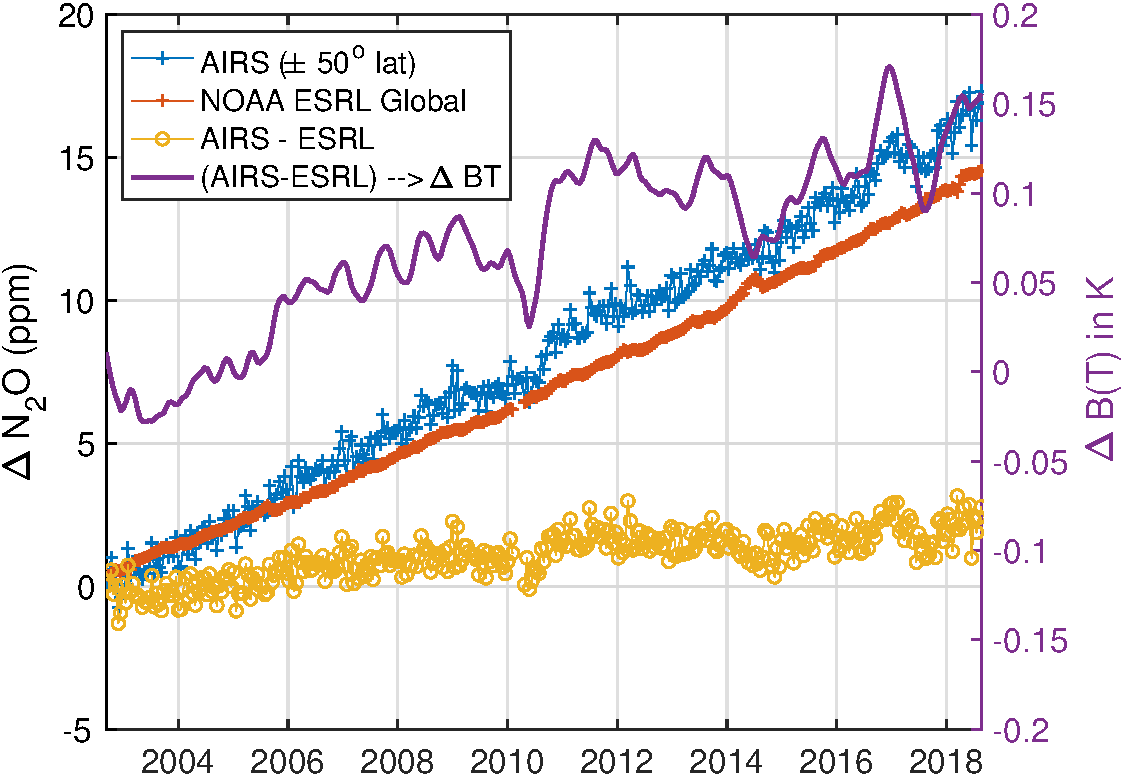
\includegraphics[width=0.7\linewidth]{./Figs/Pdf/n2o_airs_vs_esrl_global_with_dbt.pdf}
\end{center}
\end{frame}

\begin{frame}[label={sec:org95b2593}]{Pdf/ch4\_airs\_vs\_esrl\_global\_with\_dbt.pdf}
\begin{center}
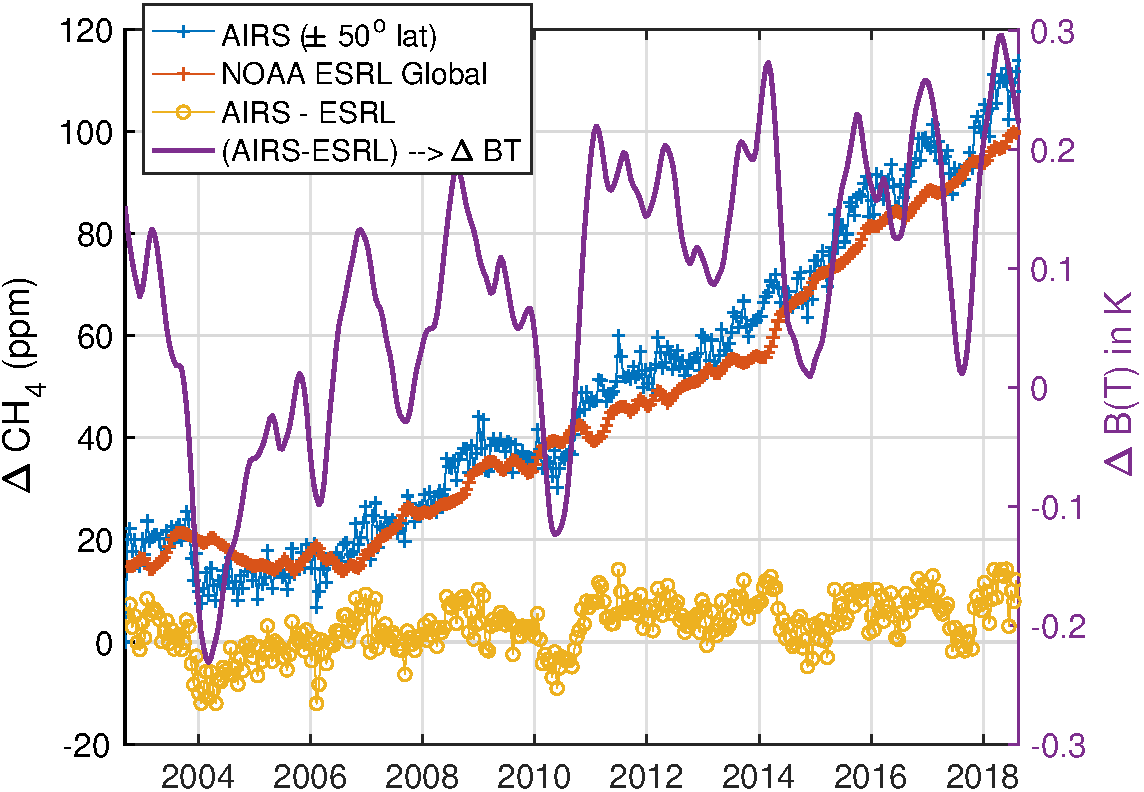
\includegraphics[width=0.7\linewidth]{./Figs/Pdf/ch4_airs_vs_esrl_global_with_dbt.pdf}
\end{center}
\end{frame}

\begin{frame}[label={sec:orgd14d823}]{Pdf/ch4\_airs\_vs\_esrl\_global\_growth\_anom.pdf}
\begin{center}
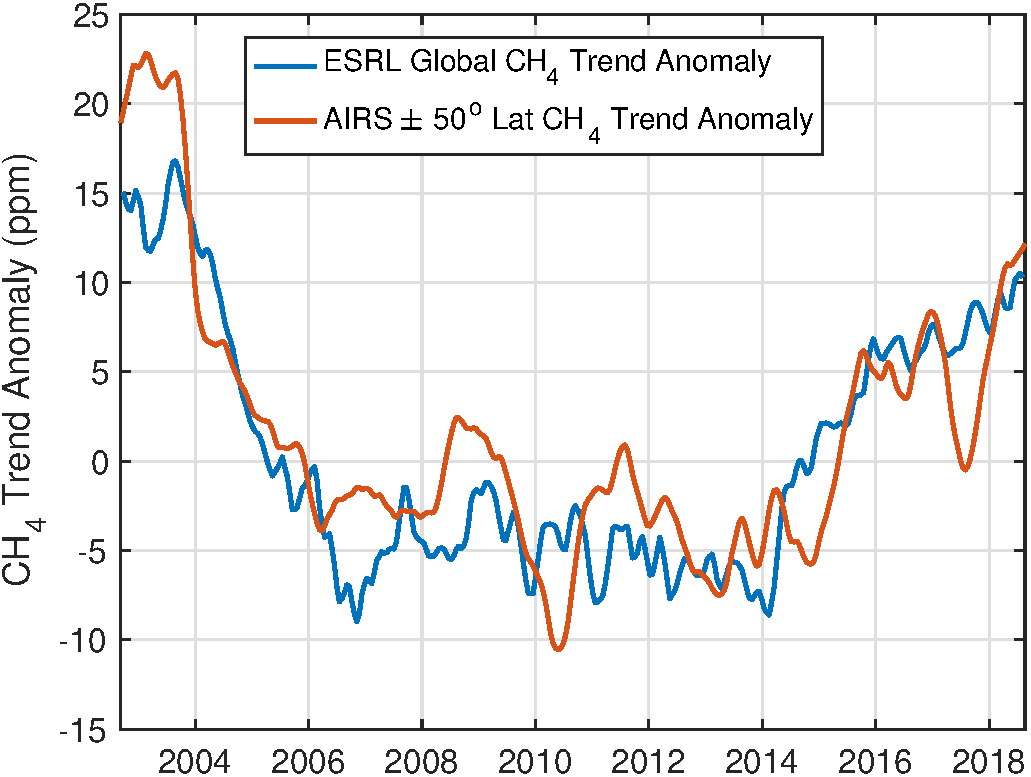
\includegraphics[width=0.7\linewidth]{./Figs/Pdf/ch4_airs_vs_esrl_global_growth_anom.pdf}
\end{center}
\end{frame}

\begin{frame}[label={sec:orgccf20b4}]{iasi\_cfc\_signatures.pdf}
\begin{center}
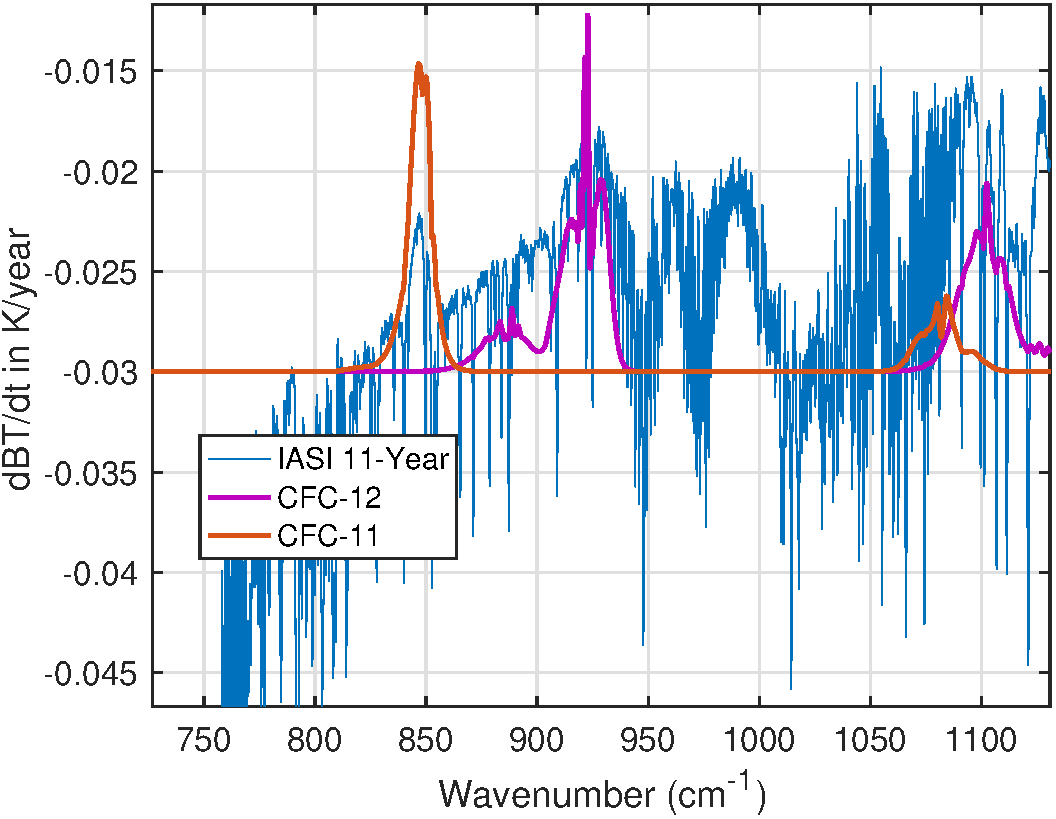
\includegraphics[width=0.7\linewidth]{./Figs/Pdf/iasi_cfc_signatures.pdf}
\end{center}
\end{frame}
\begin{frame}[label={sec:orga4af19f}]{iasi\_cfc\_bias.pdf}
\begin{center}
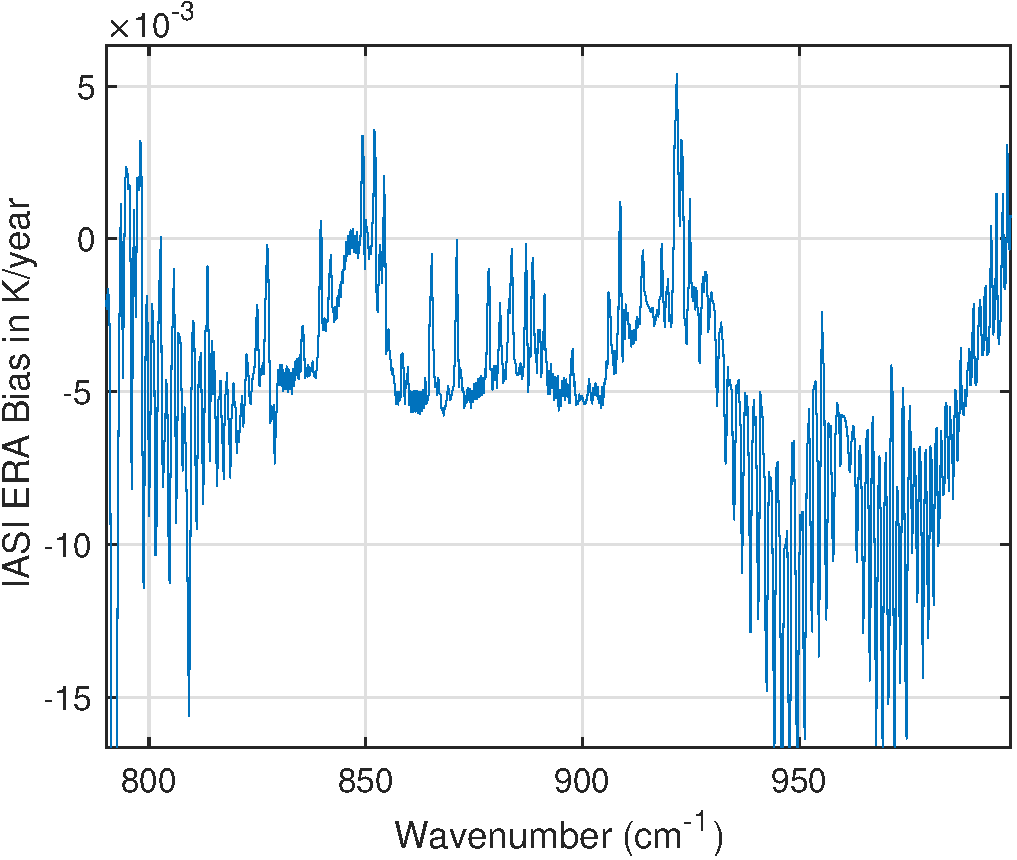
\includegraphics[width=0.7\linewidth]{./Figs/Pdf/iasi_cfc_bias.pdf}
\end{center}
\end{frame}
\begin{frame}[label={sec:org0fc707c}]{Pdf/airs\_cfc\_bias\_iasi\_times.pdf}
\begin{center}
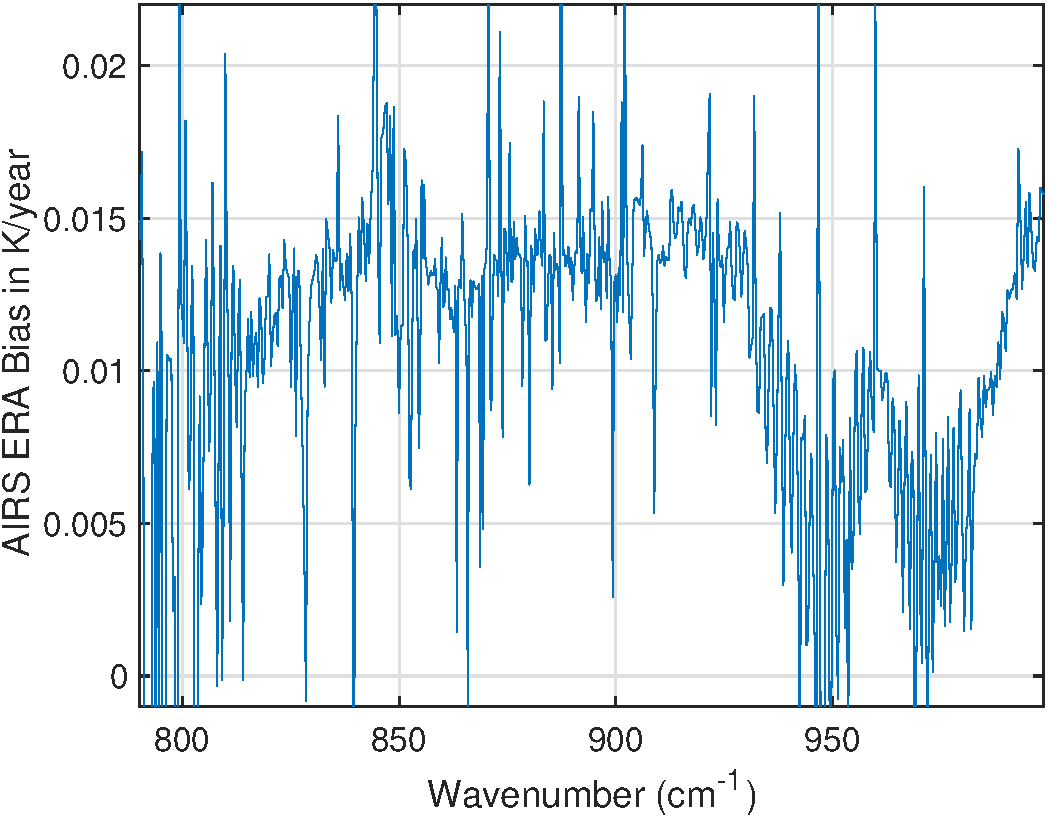
\includegraphics[width=0.7\linewidth]{./Figs/Pdf/airs_cfc_bias_iasi_times.pdf}
\end{center}
\end{frame}

\begin{frame}[label={sec:orgdc6bc2c}]{Pdf/cfc11\_bt\_trend.pdf}
\begin{center}
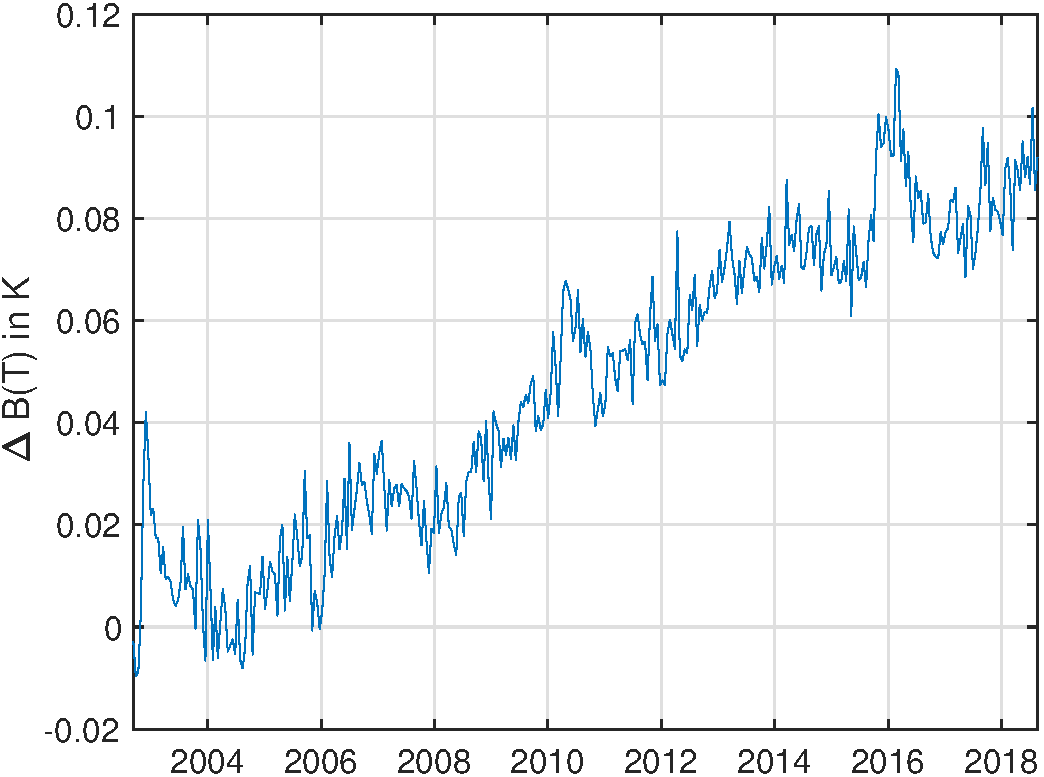
\includegraphics[width=0.7\linewidth]{./Figs/Pdf/cfc11_bt_trend.pdf}
\end{center}
\end{frame}

\begin{frame}[label={sec:org1000ebb}]{Pdf/cfc11\_trend.pdf}
\begin{center}
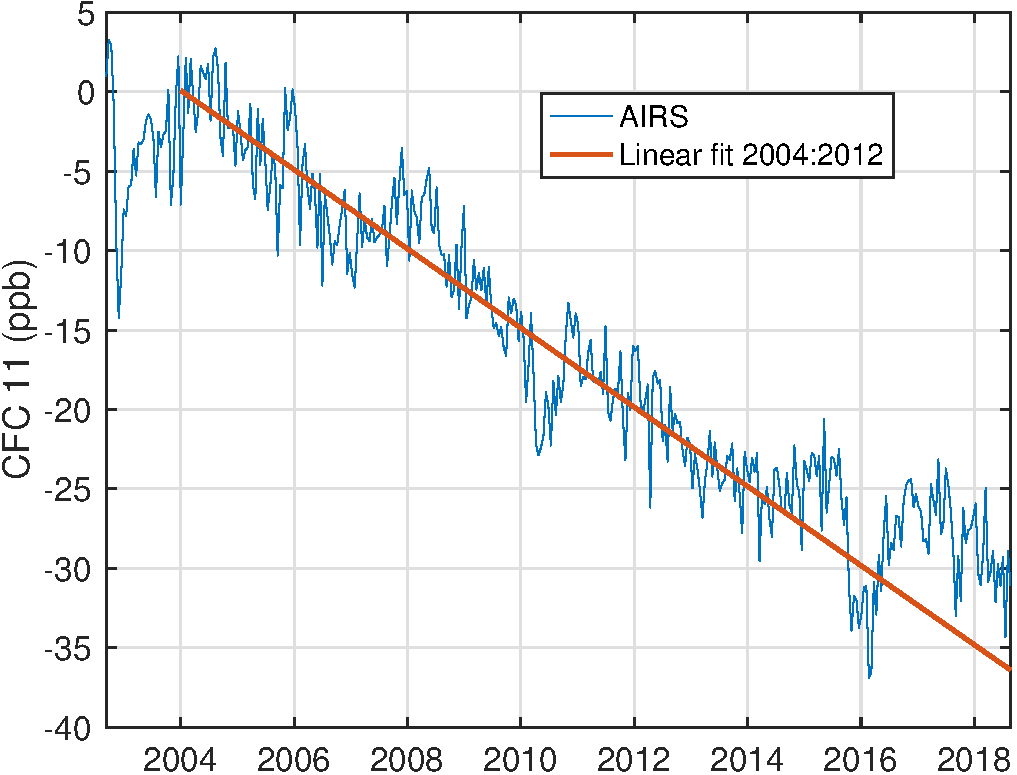
\includegraphics[width=0.7\linewidth]{./Figs/Pdf/cfc11_trend.pdf}
\end{center}
\end{frame}

\begin{frame}[label={sec:orgb82e131}]{Pdf/co2\_anom\_sst\_vs\_oisst\_clear\_sampled.pdf}
\begin{center}
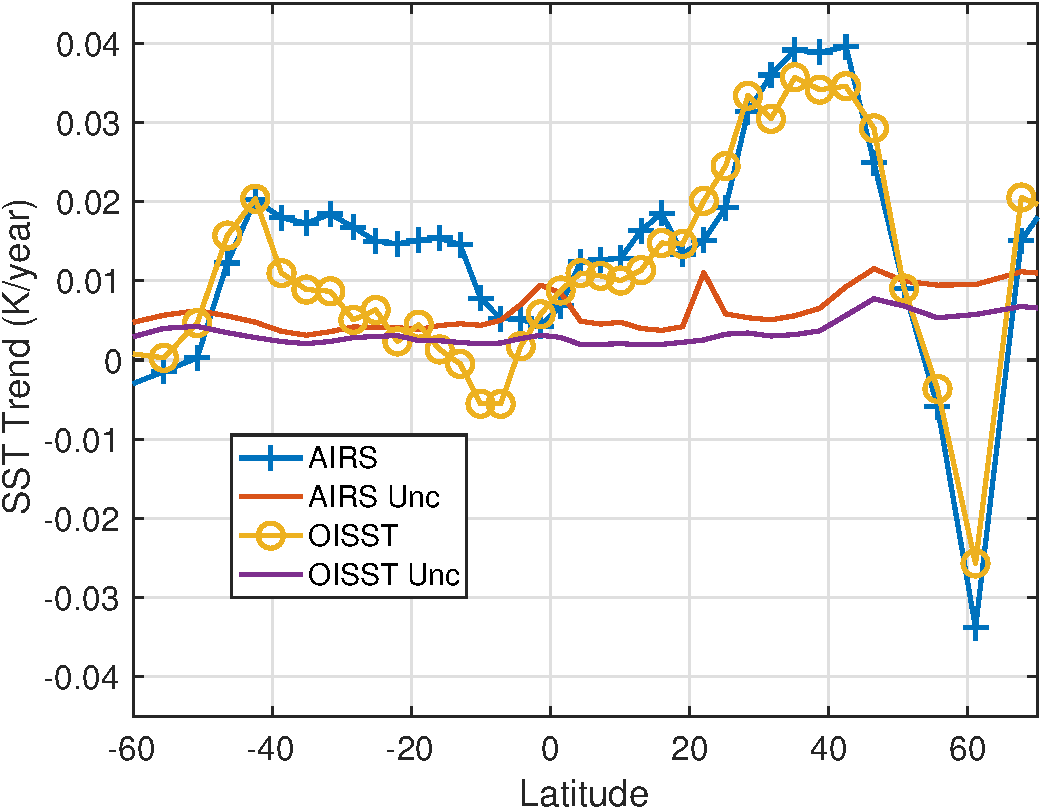
\includegraphics[width=0.7\linewidth]{./Figs/Pdf/co2_anom_sst_vs_oisst_clear_sampled.pdf}
\end{center}
\end{frame}

\begin{frame}[label={sec:org81e75bb}]{Pdf/co2\_anom\_sst\_vs\_oisst\_clear\_sampled\_and\_era.pdf}
\begin{center}
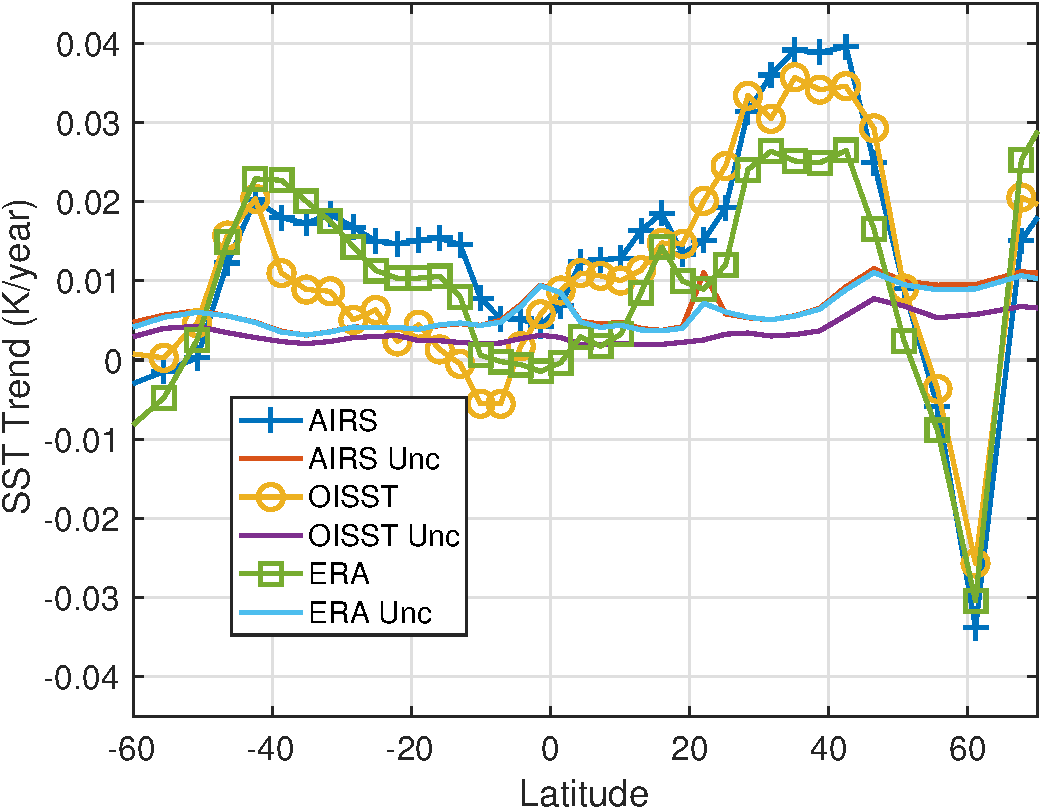
\includegraphics[width=0.7\linewidth]{./Figs/Pdf/co2_anom_sst_vs_oisst_clear_sampled_and_era.pdf}
\end{center}
\end{frame}

\begin{frame}[label={sec:org8899e57}]{Png/best\_co2\_anom\_resid.png}
\begin{center}
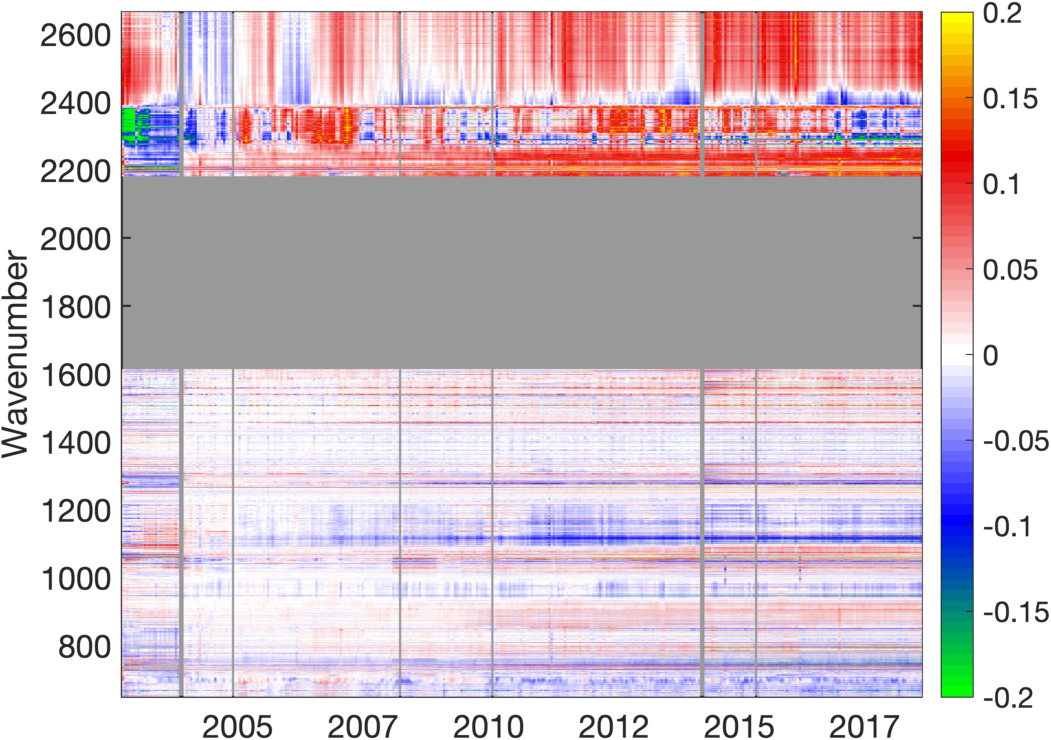
\includegraphics[width=0.7\linewidth]{./Figs/Png/best_co2_anom_resid.png}
\end{center}
\end{frame}

\begin{frame}[label={sec:org2916704}]{Png/best\_co2\_anom\_resid\_no\_sw.png}
\begin{center}
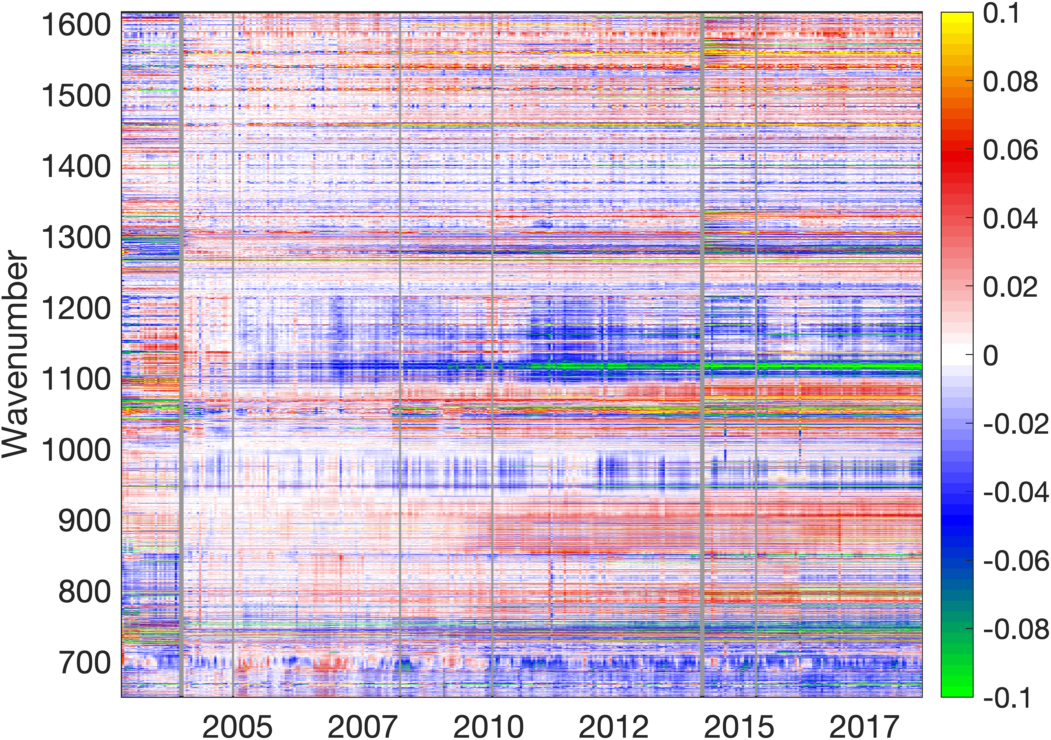
\includegraphics[width=0.7\linewidth]{./Figs/Png/best_co2_anom_resid_no_sw.png}
\end{center}
\end{frame}

\begin{frame}[label={sec:org14d8281}]{Png/best\_co2\_anomaly\_resid\_fit\_chans\_concat.png}
\begin{center}
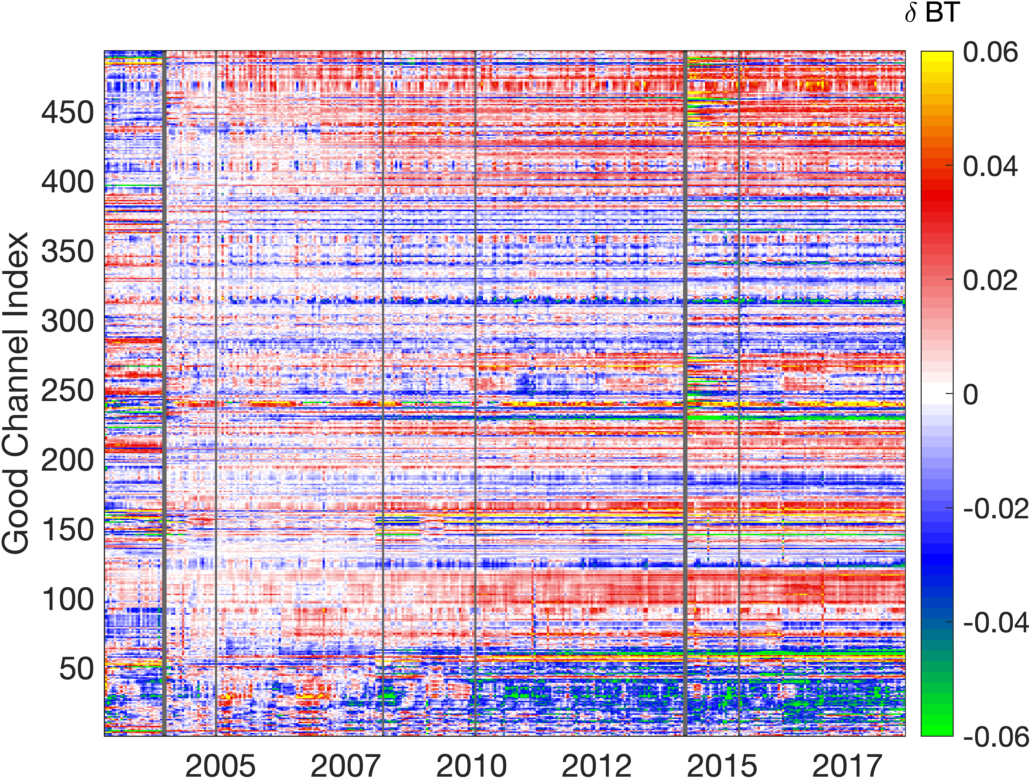
\includegraphics[width=0.7\linewidth]{./Figs/Png/best_co2_anomaly_resid_fit_chans_concat.png}
\end{center}
\end{frame}

\begin{frame}[label={sec:orgfffea2b}]{Pdf/bt\_drift\_from\_anom\_resid\_2613\_chan.pdf}
\begin{columns}
\begin{column}{0.6\columnwidth}
\begin{block}{}
\vspace{-0.3in}
\begin{center}
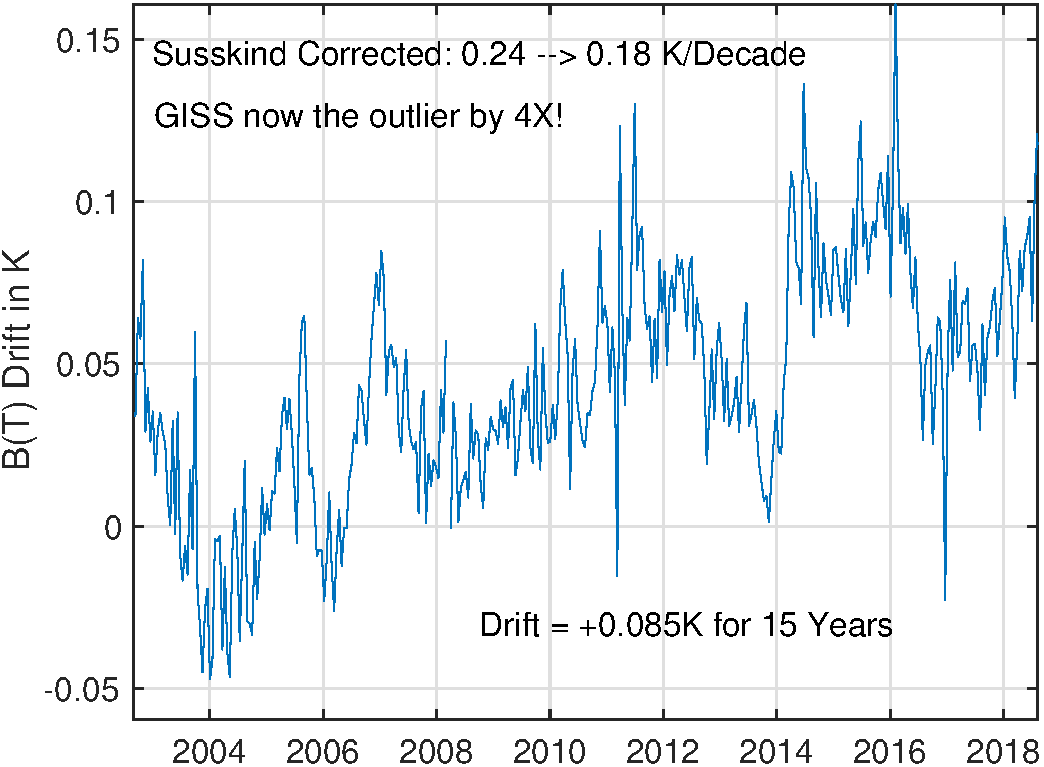
\includegraphics[width=\linewidth]{./Figs/Pdf/bt_drift_from_anom_resid_2613_chan_v2.pdf}
\end{center}
\end{block}
\end{column}

\begin{column}{0.4\columnwidth}
\begin{block}{From Susskind et. al.}
\begin{small}
\begin{center}
\begin{tabular}{ll}
AIRS & 0.24 \textpm{} 0.12\\
AIRS Corrected & 0.18\\
GISTEMP & 0.22 \textpm{} 0.13\\
HadCRUT4 & 0.17 \textpm{} 0.13\\
C\&W & 0.19 \textpm{} 0.12\\
ECMWF & 0.20 \textpm{} 0.16\\
UAH LT & 0.18\\
\end{tabular}
\end{center}
\end{small}
\end{block}
\end{column}
\end{columns}

Shortwave drift correction reduces AIRS global temperature trend by 33\% and bring AIRS into close agreement with HadCRUT4, C\&W, and UAH LT, signficantly worse agreement with GISTEMP.
\end{frame}

\begin{frame}[label={sec:org00f3965}]{Latitude Dependence Surface Trends}
\vspace{-0.3in}
\begin{columns}
\begin{column}{0.55\columnwidth}
\begin{block}{Susskind 2019: SW}
\begin{center}
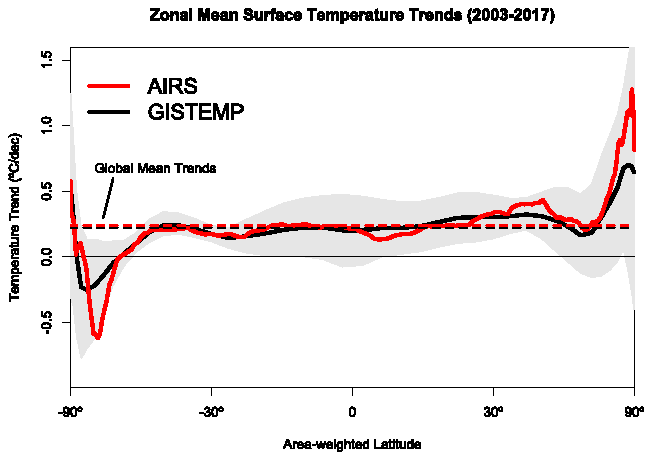
\includegraphics[width=\linewidth]{./Figs/Pdf/susskind_giss_trend_vs_lat.pdf}
\end{center}
\end{block}
\end{column}

\begin{column}{0.55\columnwidth}
\begin{block}{UMBC Trends: LW and SW}
\vspace{0.14in}
\begin{center}
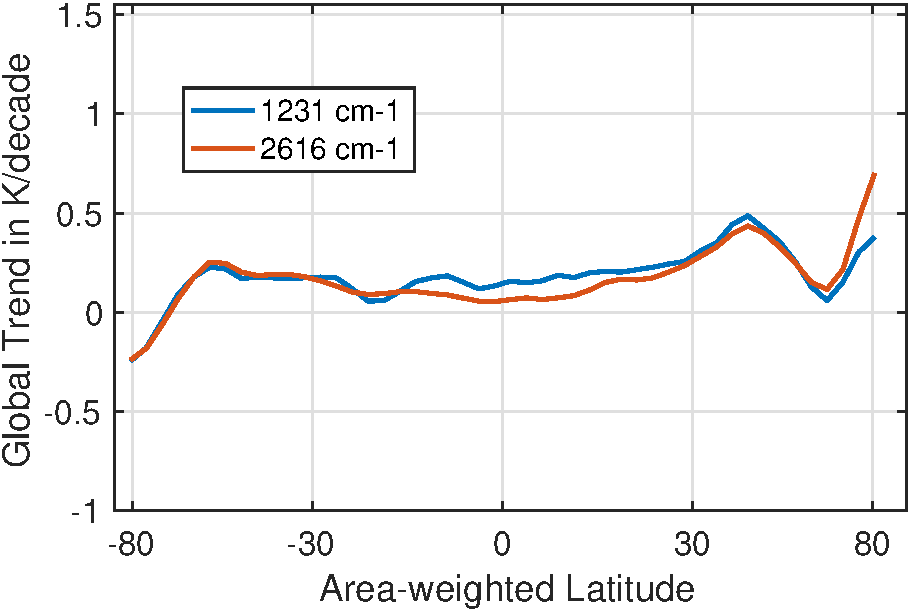
\includegraphics[width=\linewidth]{./Figs/Pdf/bt_global_trend_area_weight_lat_1231_vs_2616_from_hottest_v2.pdf}
\end{center}
\end{block}
\end{column}
\end{columns}

\vspace{-0.15in}
\begin{footnotesize}
Global Means
\begin{center}
\begin{tabular}{rrrrr}
GISS & Susskind & UMBC-1231 & UMBC-2616 & HadCRUT4\\
0.22 & 0.24 & 0.18 & 0.17 & 0.17\\
\end{tabular}
\end{center}

\vspace{-0.05in}
But, why isn't UMBC-2616 0.05K higher??\\
Note high/low Susskind values at poles not matched by UMBC\\
\emph{Rough} estimate for 2616 scene dependence: 0.06K/decade, Obs: 0.09K/decade\\
But what about the S. Pole??
\end{footnotesize}
\end{frame}

\begin{frame}[label={sec:org2bfb0f9}]{Pdf/resid\_spectrum\_dec17\_minus\_oct14\_2003.pdf}
\begin{center}
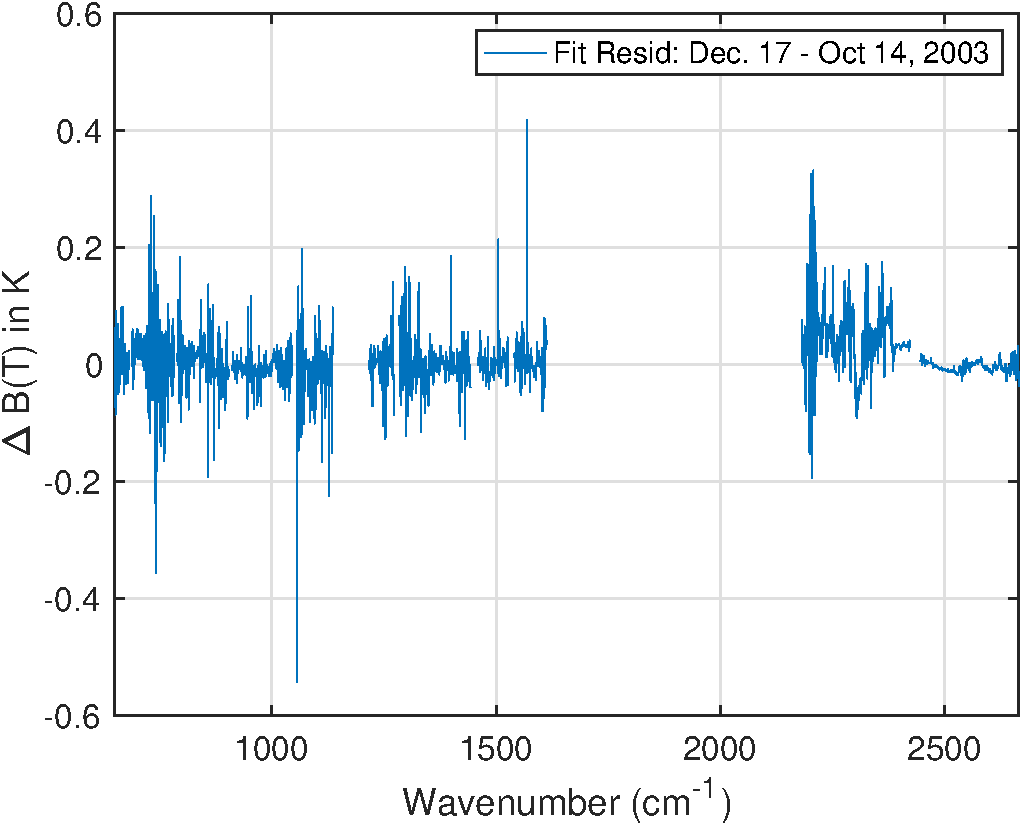
\includegraphics[width=0.7\linewidth]{./Figs/Pdf/resid_spectrum_dec17_minus_oct14_2003.pdf}
\end{center}
\end{frame}

\begin{frame}[label={sec:org7c60d00}]{Pdf/resid\_spectrum\_dec17\_minus\_oct14\_2003\_swzoom.pdf}
\begin{center}
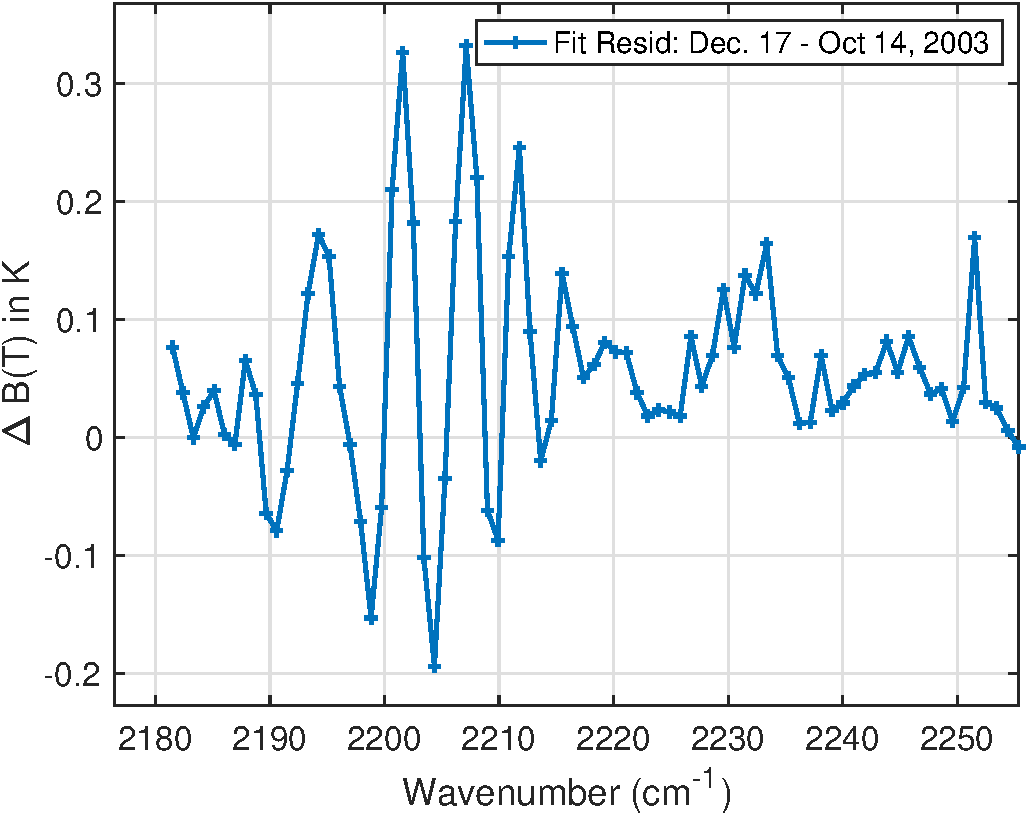
\includegraphics[width=0.7\linewidth]{./Figs/Pdf/resid_spectrum_dec17_minus_oct14_2003_swzoom.pdf}
\end{center}
\end{frame}

\begin{frame}[label={sec:org0f7b8bc}]{Pdf/resid\_1567\_and\_1570\_cm01\_dnu.pdf}
\begin{center}
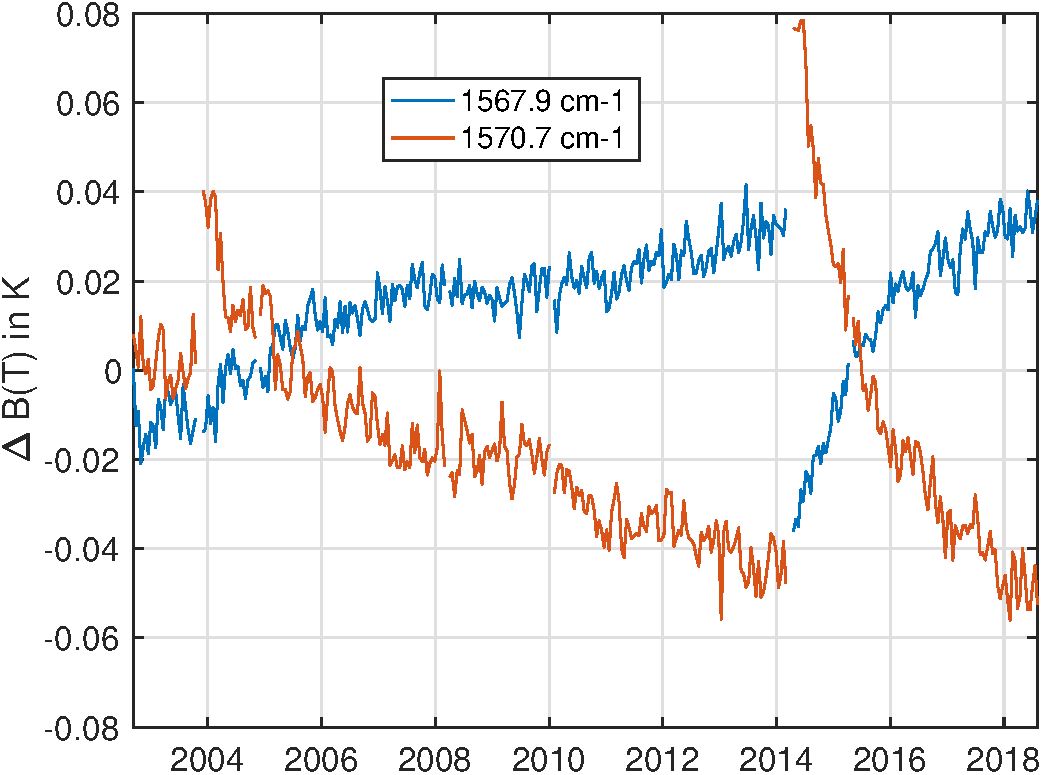
\includegraphics[width=0.7\linewidth]{./Figs/Pdf/resid_1567_and_1570_cm01_dnu.pdf}
\end{center}
\end{frame}

\begin{frame}[label={sec:orga782a80}]{DCC1}
\begin{figure}[htbp]
\centering
\includegraphics[width=0.7\linewidth]{./Figsdc/Pdf/bt2616_and_bt960_dcc_vs_time_airs_and_iasi.pdf}
\caption{\emph{AIRS and IASI Dcc daily average temperatures versus time.  The IASI curve for 2616 cm\textsuperscript{-1} is an average over 54 IASI channels.}}
\end{figure}
\end{frame}

\begin{frame}[label={sec:org0a3d5fd}]{DCC4}
\begin{figure}[htbp]
\centering
\includegraphics[width=0.7\linewidth]{./Figsdc/Pdf/airs_iasi_dcc_rate_sw_iasi_avgpts.pdf}
\caption{\emph{Same as Fig. where? with every two points in IASI averaged.}}
\end{figure}
\end{frame}

\begin{frame}[label={sec:org4c4dfcc}]{DCC6}
\begin{figure}[htbp]
\centering
\includegraphics[width=0.7\linewidth]{./Figsdc/Pdf/airs_iasi_dcc_rate_lw_ab_diffs_vs_iasi.pdf}
\caption{\emph{Longwave DCC linear rate of change with AIRS A,B, AB channels identifications highlighted.}}
\end{figure}
\end{frame}


\begin{frame}[label={sec:orgd8d380b}]{overroye\_scan.pdf}
\begin{center}
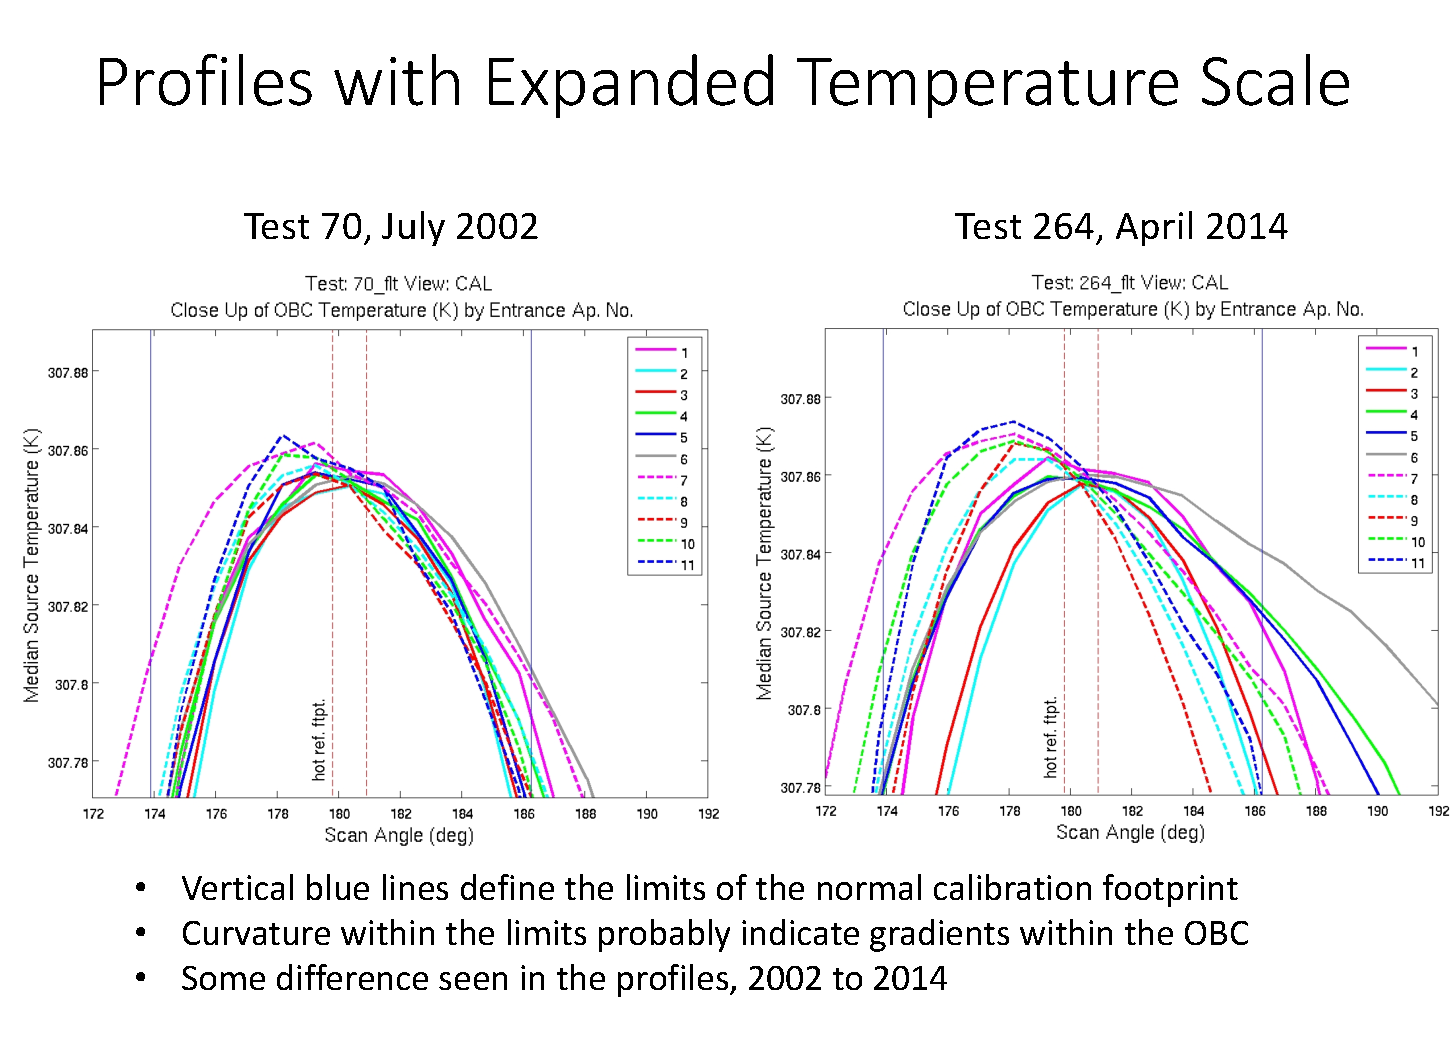
\includegraphics[width=0.7\linewidth]{./Figs/Pdf/overroye_scan.pdf}
\end{center}
\end{frame}

\begin{frame}[label={sec:orgd1192b7}]{overroye\_map.pdf}
\begin{center}
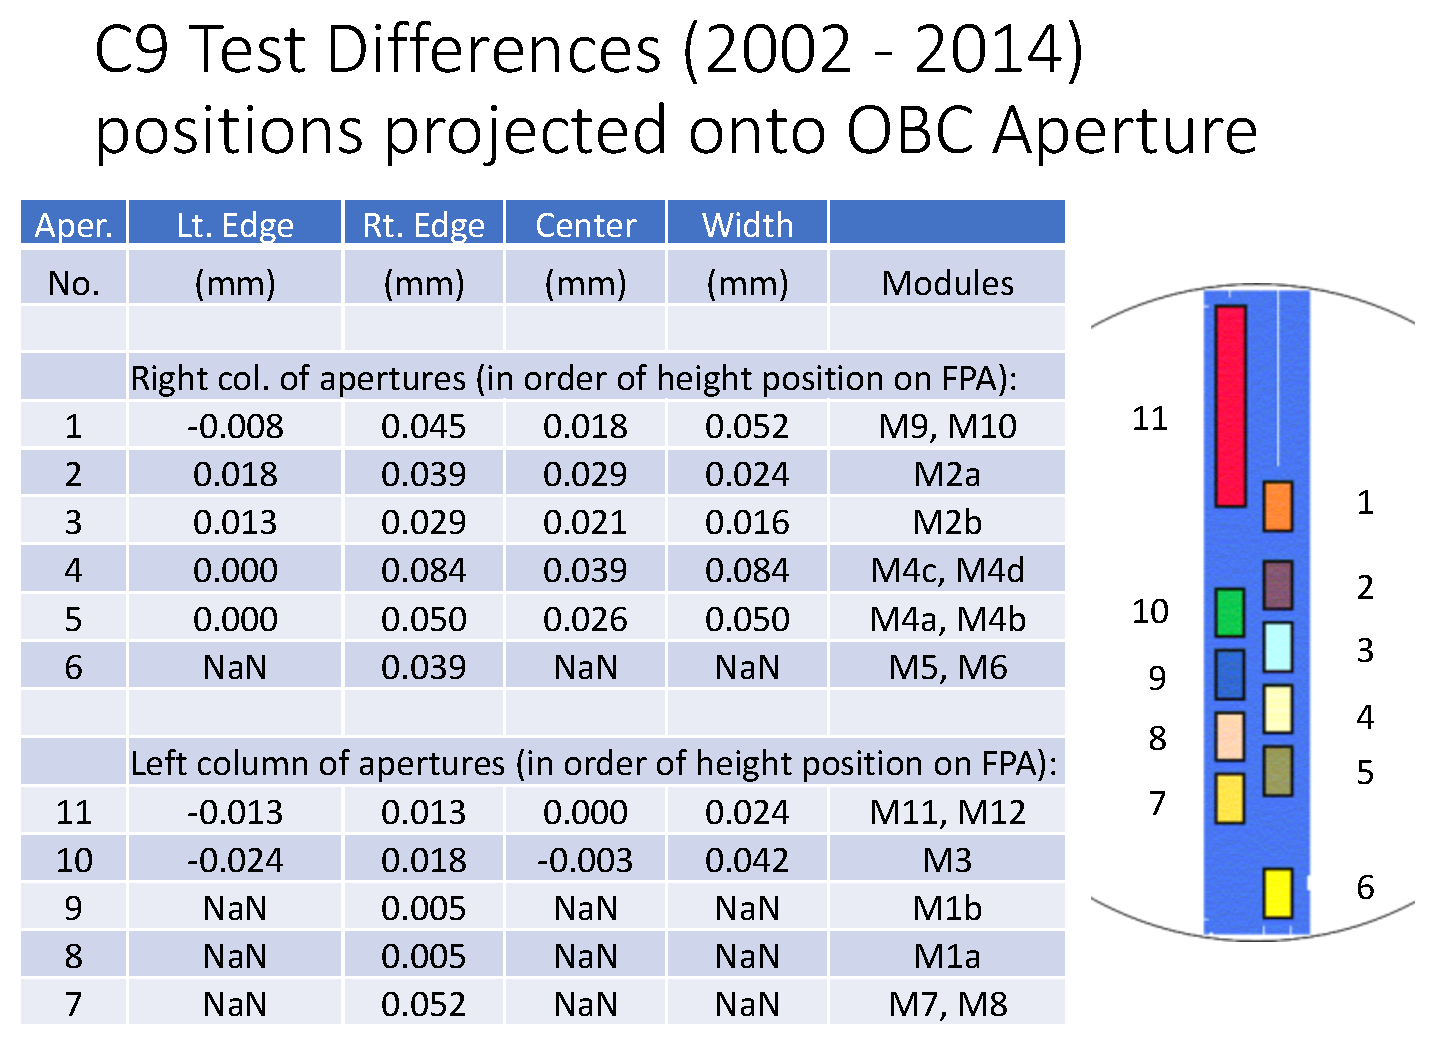
\includegraphics[width=0.7\linewidth]{./Figs/Pdf/overroye_map.pdf}
\end{center}
\end{frame}


\begin{frame}[label={sec:orgd686cb6}]{Surface T Trends Using 1231 \wn Channel}
\vspace{-0.35in}

\begin{columns}
\begin{column}{0.55\columnwidth}
\begin{block}{\footnotesize AIRS 1231 \wn}
\vspace{-0.1in}
\begin{center}
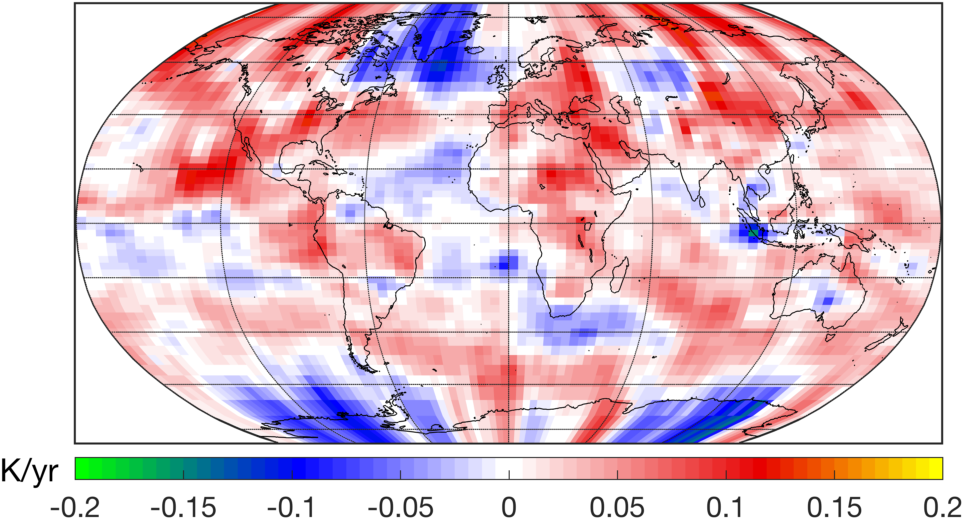
\includegraphics[width=\linewidth]{./Figs/Png/airs_tsurf_trend_from_1231cm_trend.png}
\end{center}
\end{block}
\end{column}

\begin{column}{0.55\columnwidth}
\begin{block}{\footnotesize ERA}
\vspace{-0.1in}
\begin{center}
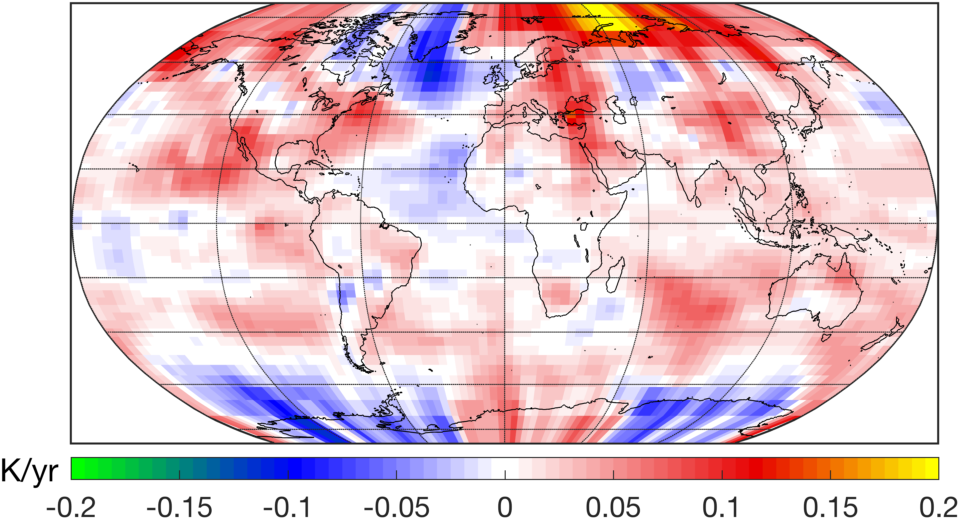
\includegraphics[width=\linewidth]{./Figs/Png/era_tsurf_trend.png}
\end{center}
\end{block}
\end{column}
\end{columns}


\begin{columns}
\begin{column}{0.55\columnwidth}
\begin{block}{\footnotesize OISST}
\vspace{-0.1in}
\begin{center}
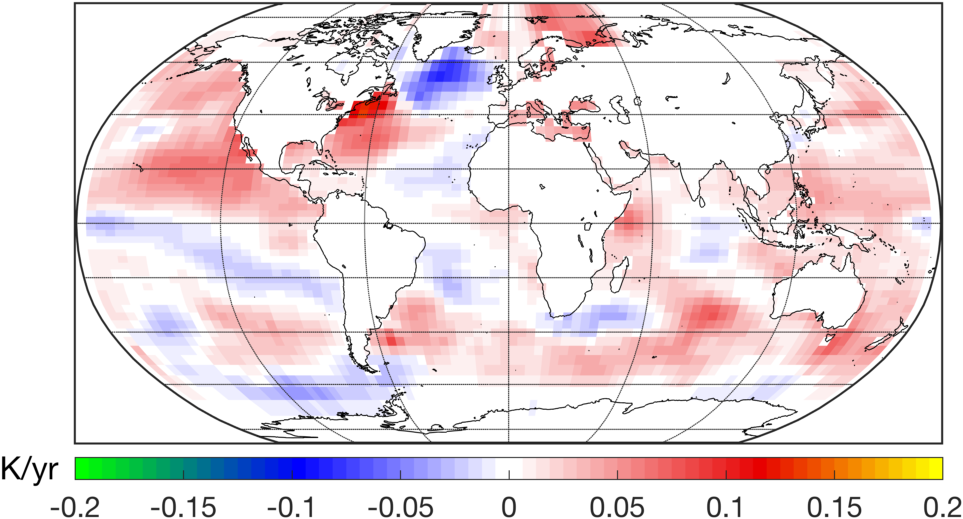
\includegraphics[width=\linewidth]{./Figs/Png/oisst_trend_map.png}
\end{center}
\end{block}
\end{column}

\begin{column}{0.5\columnwidth}
\begin{block}{\footnotesize AIRS 2616 \wn}
\vspace{-0.1in}
\begin{center}
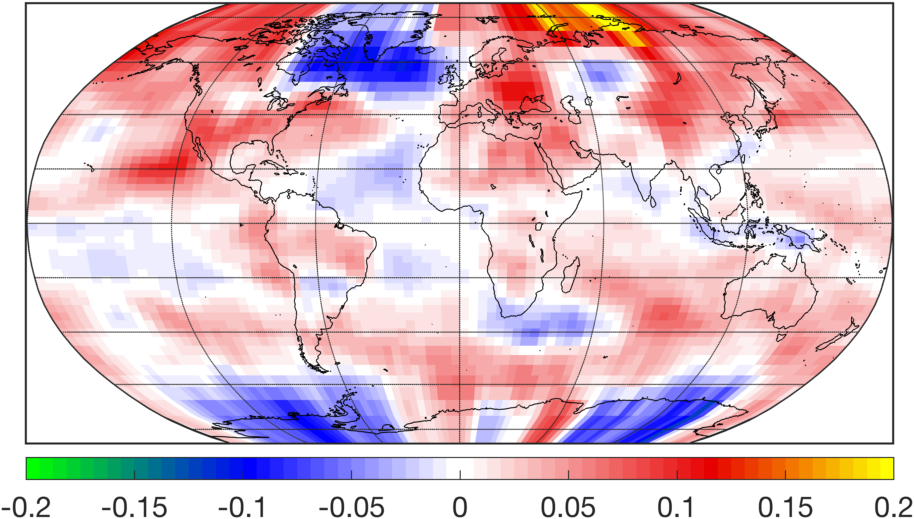
\includegraphics[width=\linewidth]{./Figs/Png/airs_tsurf_trend_from_2616cm_trend.png}
\end{center}
\end{block}
\end{column}
\end{columns}
\end{frame}


\begin{frame}[label={sec:orgc70f088}]{Pdf/zonal\_sst\_trends\_12311\_vs\_oisst\_ersst5\_hottest\_per\_grid\_envelope.pdf}
\begin{center}
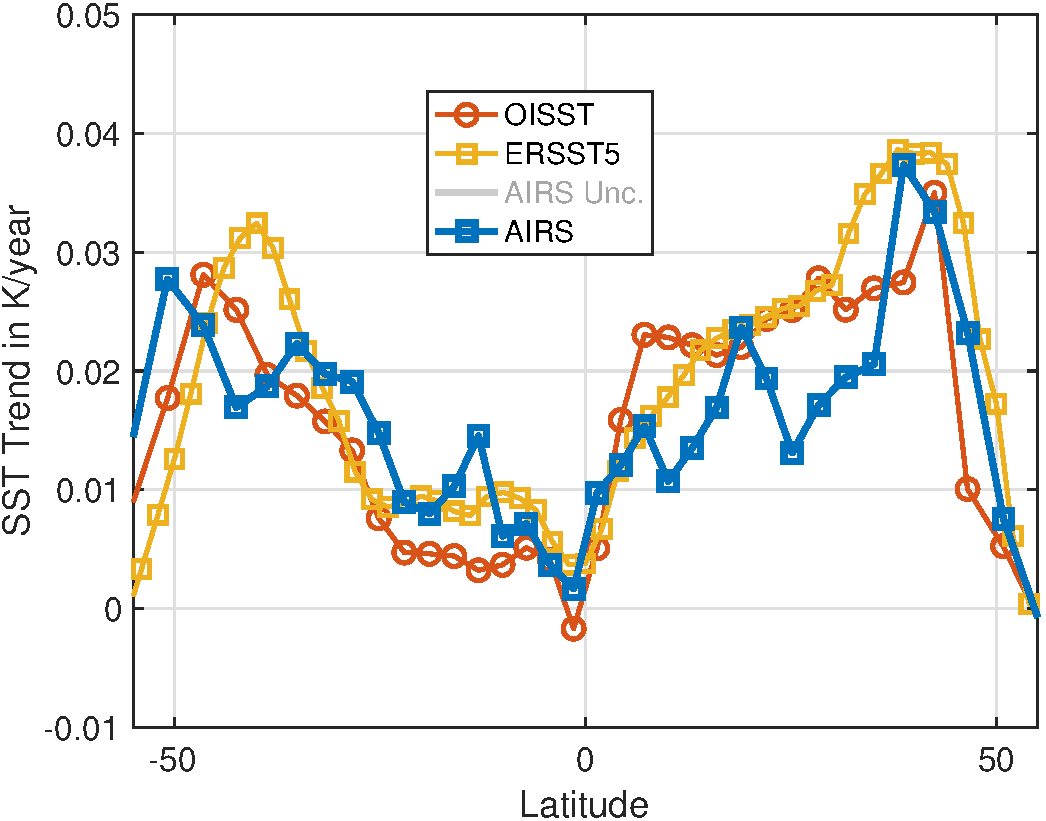
\includegraphics[width=0.7\linewidth]{./Figs/Pdf/zonal_sst_trends_12311_vs_oisst_ersst5_hottest_per_grid_envelope.pdf}
\end{center}
\end{frame}
\begin{frame}[label={sec:orgd0b9c54}]{Cloud Forcing Zonal Trends}
\vspace{-0.3in}

\begin{columns}
\begin{column}{0.33\columnwidth}
\begin{block}{\footnotesize Some Small Title}
\vspace{0.0in}
\begin{center}
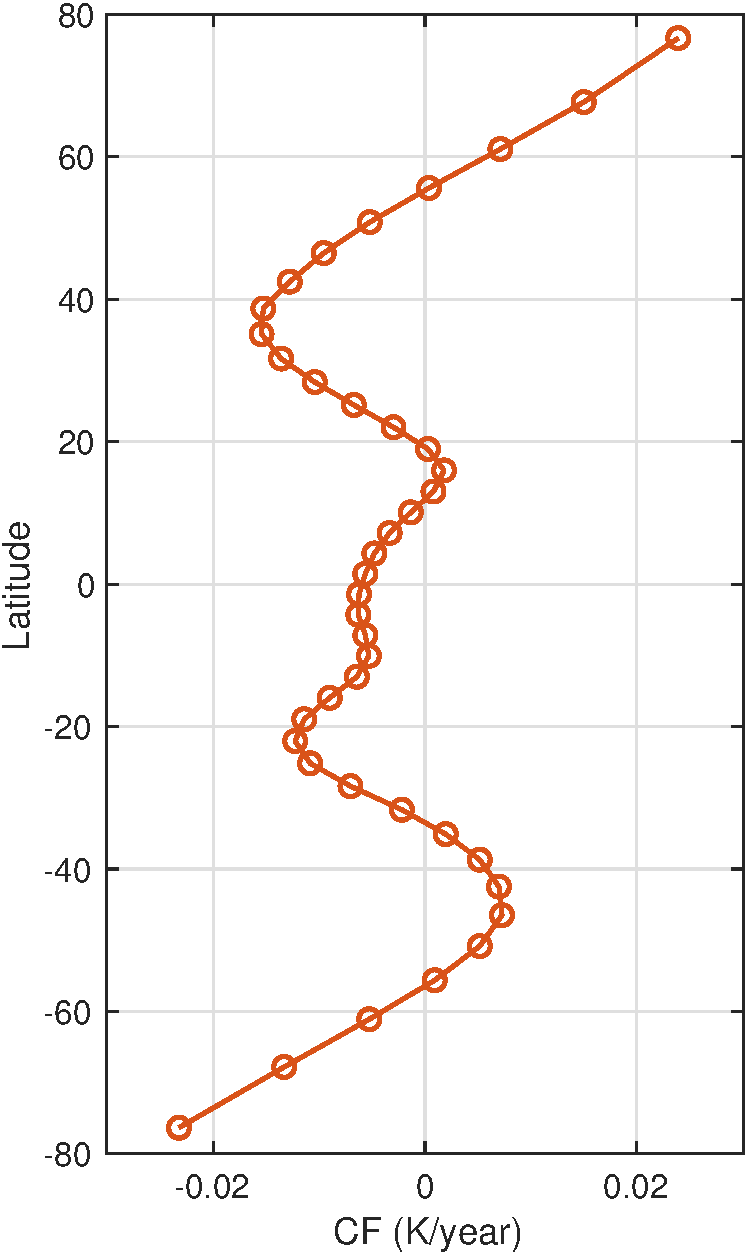
\includegraphics[width=\linewidth]{./Figs/Pdf/new_trend_rand_stats_1231_and_2161_era_clr_minus_obs_smoothed.pdf}
\end{center}
\end{block}
\end{column}

\begin{column}{0.33\columnwidth}
\begin{block}{\footnotesize Another Small Title}
\vspace{-0.1in}
\begin{center}
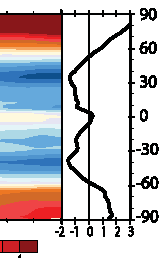
\includegraphics[width=\linewidth]{./Figs/Pdf/trenberth_total_only.pdf}
\end{center}
\end{block}
\end{column}

\begin{column}{0.33\columnwidth}
\begin{block}{\footnotesize Another Small Title}
\vspace{-0.1in}
\begin{center}
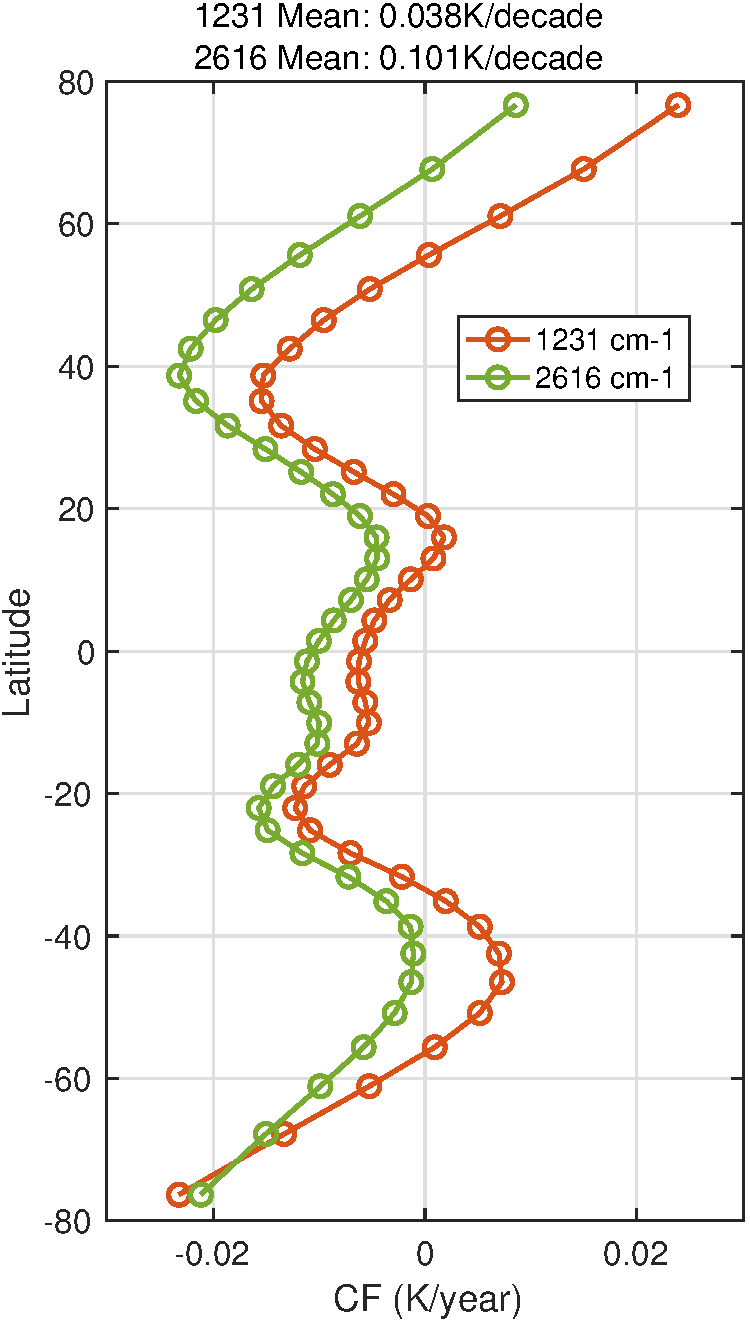
\includegraphics[width=\linewidth]{./Figs/Pdf/new_trend_rand_stats_1231_and_2161_era_clr_minus_obs_smoothed_with_2616_labelled.pdf}
\end{center}
\end{block}
\end{column}
\end{columns}
\end{frame}

\begin{frame}[label={sec:org46bbc2c}]{Pdf/new\_trend\_rand\_stats\_1231\_and\_2161\_era\_clr\_minus\_obs\_smoothed.pdf}
\begin{center}
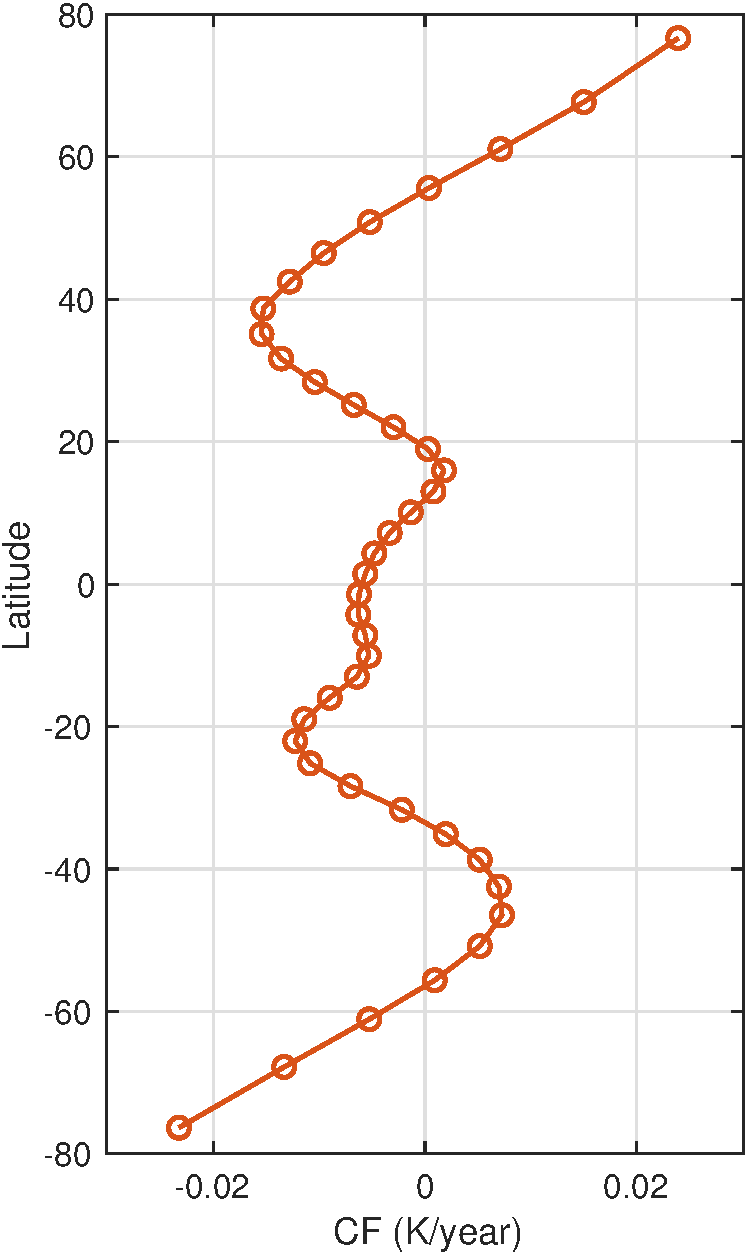
\includegraphics[width=0.4\linewidth]{./Figs/Pdf/new_trend_rand_stats_1231_and_2161_era_clr_minus_obs_smoothed.pdf}
\end{center}
\end{frame}

\begin{frame}[label={sec:org6a936c9}]{Pdf/new\_trend\_rand\_stats\_1231\_and\_2161\_era\_clr\_minus\_obs\_smoothed\_with\_2616\_labelled.pdf}
\begin{center}
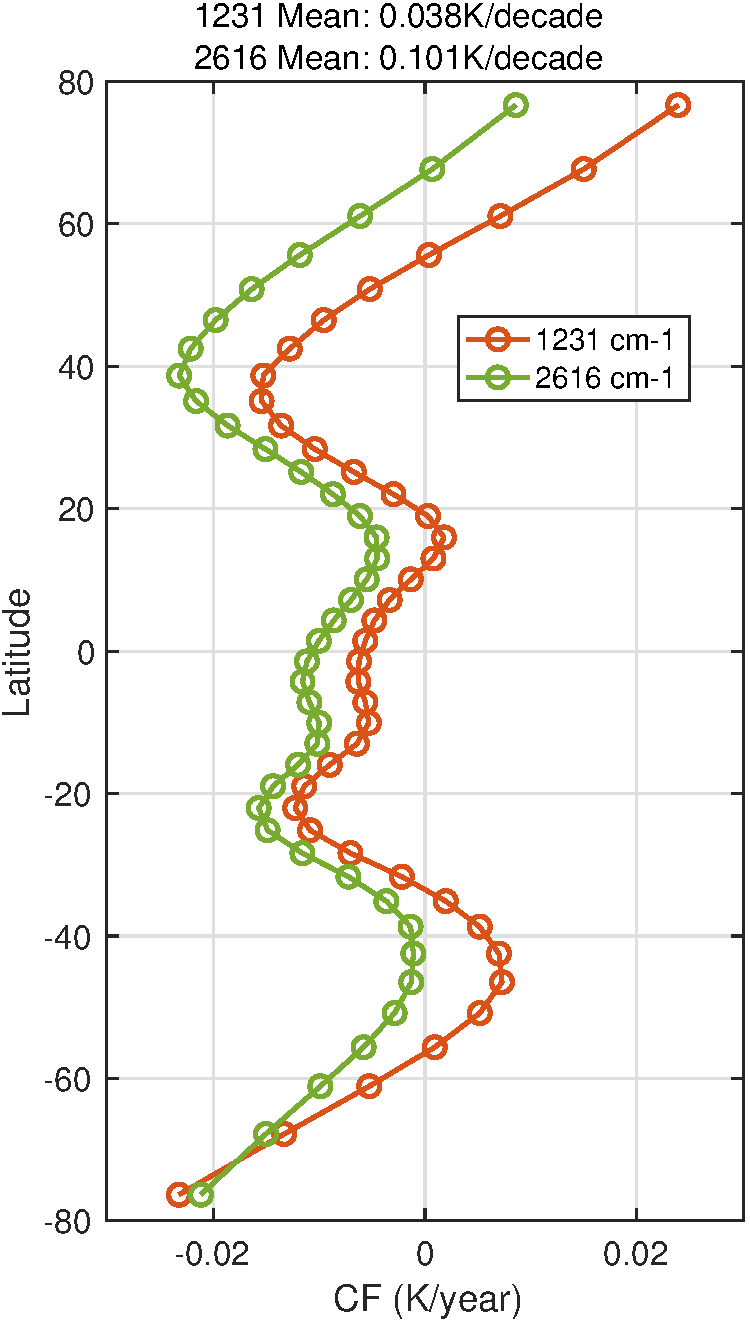
\includegraphics[width=0.4\linewidth]{./Figs/Pdf/new_trend_rand_stats_1231_and_2161_era_clr_minus_obs_smoothed_with_2616_labelled.pdf}
\end{center}
\end{frame}
\begin{frame}[label={sec:org45ac550}]{Pdf/trenberth\_total\_only.pdf}
\begin{center}
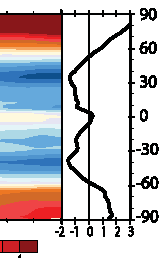
\includegraphics[width=0.7\linewidth]{./Figs/Pdf/trenberth_total_only.pdf}
\end{center}
\end{frame}

\begin{frame}[label={sec:orgd04b00e}]{Pdf/trenberth2009\_clouds\_top.pdf}
\begin{center}
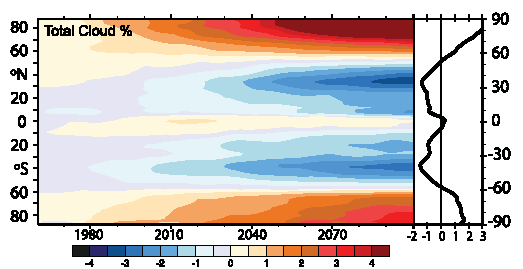
\includegraphics[width=0.7\linewidth]{./Figs/Pdf/trenberth2009_clouds_top.pdf}
\end{center}
\end{frame}

\begin{frame}[label={sec:orgaf52848}]{Pdf/trenberth2009\_clouds.pdf}
\begin{center}
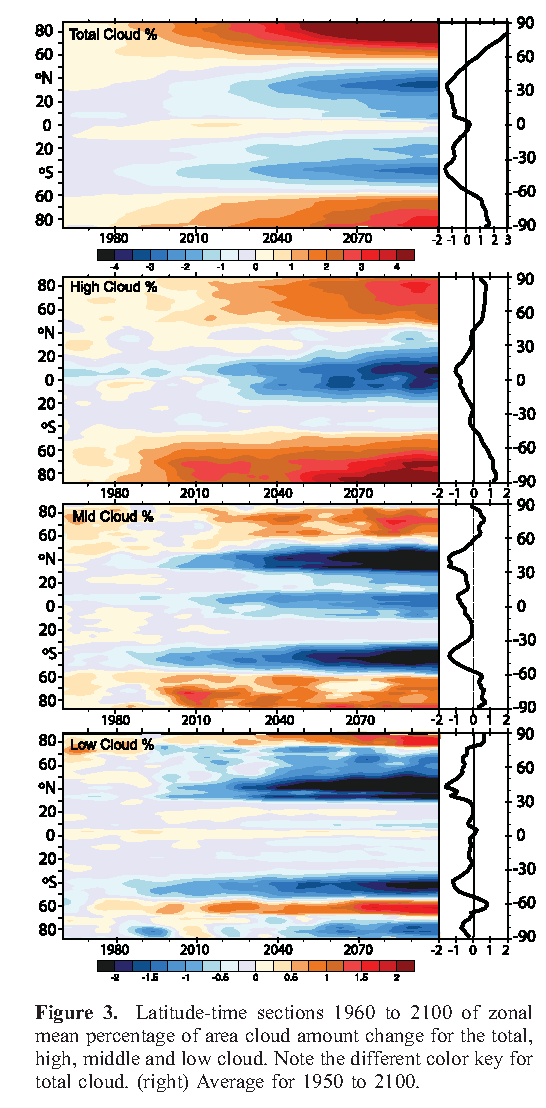
\includegraphics[width=0.7\linewidth]{./Figs/Pdf/trenberth2009_clouds.pdf}
\end{center}
\end{frame}

\begin{frame}[label={sec:org86dcffe}]{Pdf/tseries\_sst\_obs\_global.pdf}
\begin{center}
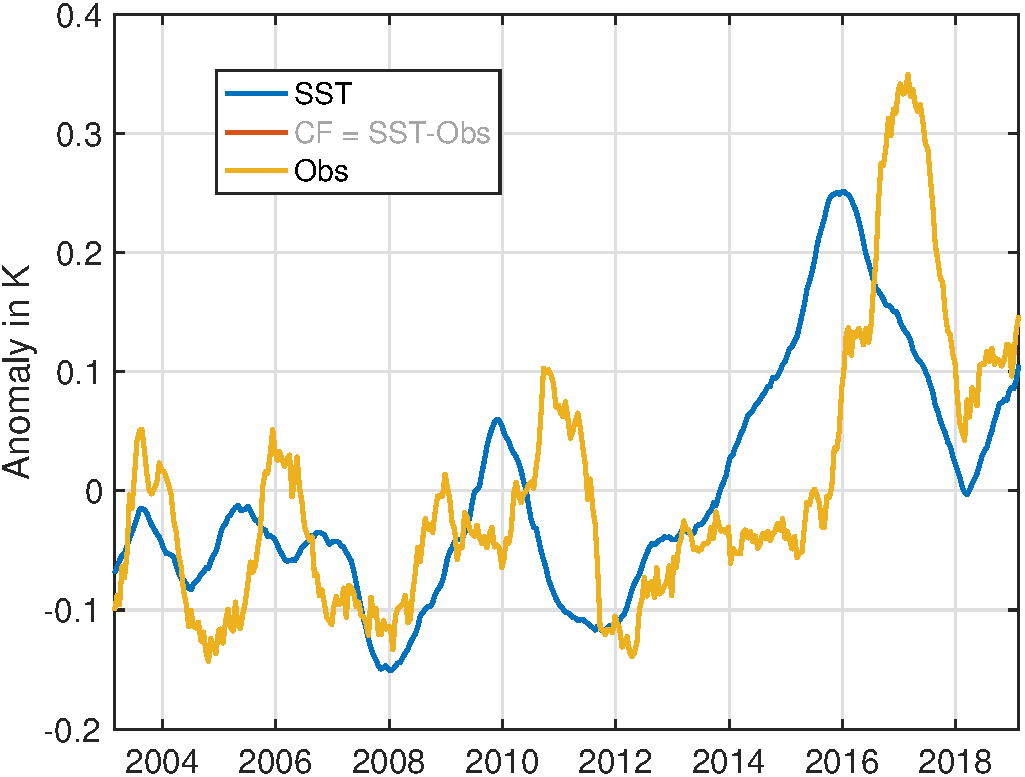
\includegraphics[width=0.7\linewidth]{./Figs/Pdf/tseries_sst_obs_global.pdf}
\end{center}
\end{frame}

\begin{frame}[label={sec:org6885406}]{Pdf/tseries\_sst\_cf\_obs\_global.pdf}
\begin{center}
\includegraphics[width=0.7\linewidth]{./Figs/Pdf/tseries_sst_cf_obs_global.pdf}
\end{center}
\end{frame}

\begin{frame}[label={sec:org2eddeee}]{Pdf/ocean\_btobs\_delay\_from\_sst.pdf}
\begin{center}
\includegraphics[width=0.7\linewidth]{./Figs/Pdf/ocean_btobs_delay_from_sst.pdf}
\end{center}
\end{frame}

\begin{frame}[label={sec:orgfb11446}]{Pdf/cf\_vs\_sst\_vs\_year\_2019.pdf}
\begin{center}
\includegraphics[width=0.7\linewidth]{./Figs/Pdf/cf_vs_sst_vs_year_2019.pdf}
\end{center}
\end{frame}

\begin{frame}[label={sec:org14249b8}]{Pdf/cf\_vs\_sst\_vs\_enso\_v2.pdf}
\begin{center}
\includegraphics[width=0.7\linewidth]{./Figs/Pdf/cf_vs_sst_vs_enso_v2.pdf}
\end{center}
\end{frame}

\begin{frame}[label={sec:org356c368}]{Pdf/lw\_h2o\_flux\_kernel.pdf}
\begin{center}
\includegraphics[width=0.7\linewidth]{./Figs/Pdf/lw_h2o_flux_kernel.pdf}
\end{center}
\end{frame}

\begin{frame}[label={sec:org66114b2}]{Png/water\_chans\_1400to1600\_trend\_vs\_btobs\_2dhist\_global.png}
\begin{center}
\includegraphics[width=0.7\linewidth]{./Figs/Png/water_chans_1400to1600_trend_vs_btobs_2dhist_global.png}
\end{center}
\end{frame}
\end{document}